%% Based on a TeXnicCenter-Template by Tino Weinkauf.
%%%%%%%%%%%%%%%%%%%%%%%%%%%%%%%%%%%%%%%%%%%%%%%%%%%%%%%%%%%%%

%%%%%%%%%%%%%%%%%%%%%%%%%%%%%%%%%%%%%%%%%%%%%%%%%%%%%%%%%%%%%
%% HEADER
%%%%%%%%%%%%%%%%%%%%%%%%%%%%%%%%%%%%%%%%%%%%%%%%%%%%%%%%%%%%%
\documentclass[a4paper,oneside,12pt]{report}
% Alternative Options:
%	Paper Size: a4paper / a5paper / b5paper / letterpaper / legalpaper / executivepaper
% Duplex: oneside / twoside
% Base Font Size: 10pt / 11pt / 12pt


%% Language %%%%%%%%%%%%%%%%%%%%%%%%%%%%%%%%%%%%%%%%%%%%%%%%%
\usepackage[USenglish]{babel}
\usepackage[ansinew,latin5]{inputenc}
\usepackage[T1]{fontenc}
\usepackage{lmodern} %Type1-font for non-english texts and characters
\usepackage[top=3cm, bottom=3cm,left=4cm,right=2cm]{geometry}
\usepackage{graphicx}
\usepackage{wrapfig}
\usepackage{parskip}

\usepackage{setspace}
\usepackage{caption}
\usepackage{subcaption}
\usepackage{amssymb}

%% Packages for Graphics & Figures %%%%%%%%%%%%%%%%%%%%%%%%%%
\usepackage{graphicx} %%For loading graphic files
\usepackage{subfig} %%Subfigures inside a figure
%\usepackage{tikz} %%Generate vector graphics from within LaTeX
\usepackage[toc,page]{appendix}
%% Please note:
%% Images can be included using \includegraphics{filename}
%% resp. using the dialog in the Insert menu.
%% 
%% The mode "LaTeX => PDF" allows the following formats:
%%   .jpg  .png  .pdf  .mps
%% 
%% The modes "LaTeX => DVI", "LaTeX => PS" und "LaTeX => PS => PDF"
%% allow the following formats:
%%   .eps  .ps  .bmp  .pict  .pntg


%% Math Packages %%%%%%%%%%%%%%%%%%%%%%%%%%%%%%%%%%%%%%%%%%%%
\usepackage{amsmath}
\usepackage{amsthm}
\usepackage{amsfonts}
\usepackage{algorithm}
\usepackage{algpseudocode}
\algnewcommand\myAnd{\textbf{and}}

%% Line Spacing %%%%%%%%%%%%%%%%%%%%%%%%%%%%%%%%%%%%%%%%%%%%%
\usepackage{setspace}
%\singlespacing        %% 1-spacing (default)
\onehalfspacing       %% 1,5-spacing
%\doublespacing        %% 2-spacing


%% Other Packages %%%%%%%%%%%%%%%%%%%%%%%%%%%%%%%%%%%%%%%%%%%
%\usepackage{a4wide} %%Smaller margins = more text per page.
%\usepackage{fancyhdr} %%Fancy headings
%\usepackage{longtable} %%For tables, that exceed one page


%%%%%%%%%%%%%%%%%%%%%%%%%%%%%%%%%%%%%%%%%%%%%%%%%%%%%%%%%%%%%
%% Remarks
%%%%%%%%%%%%%%%%%%%%%%%%%%%%%%%%%%%%%%%%%%%%%%%%%%%%%%%%%%%%%
%
% TODO:
% 1. Edit the used packages and their options (see above).
% 2. If you want, add a BibTeX-File to the project
%    (e.g., 'literature.bib').
% 3. Happy TeXing!
%
%%%%%%%%%%%%%%%%%%%%%%%%%%%%%%%%%%%%%%%%%%%%%%%%%%%%%%%%%%%%%

%%%%%%%%%%%%%%%%%%%%%%%%%%%%%%%%%%%%%%%%%%%%%%%%%%%%%%%%%%%%%
%% Options / Modifications
%%%%%%%%%%%%%%%%%%%%%%%%%%%%%%%%%%%%%%%%%%%%%%%%%%%%%%%%%%%%%

%\input{options} %You need a file 'options.tex' for this
%% ==> TeXnicCenter supplies some possible option files
%% ==> with its templates (File | New from Template...).


\hyphenation{ba-�a-r�-s� i-�e-ri-sin-de �e-kil-de h�c-re-ler-den bo-yut-lu ba�-lan-g�� se-�il-mi� B�-l�m Ba�-lan-g��-ta a-ra-s�n-da saf-ha-da ge-�i-len ya-ra-t�l-m��-t�r sa�-la-n�-yor-sa si-m�-las-yon}
%%%%%%%%%%%%%%%%%%%%%%%%%%%%%%%%%%%%%%%%%%%%%%%%%%%%%%%%%%%%%
%% DOCUMENT
%%%%%%%%%%%%%%%%%%%%%%%%%%%%%%%%%%%%%%%%%%%%%%%%%%%%%%%%%%%%%
\begin{document}

%% The nice version:
%\input{titlepage} %%You need a file 'titlepage.tex' for this.
%% ==> TeXnicCenter supplies a possible titlepage file
%% ==> with its templates (File | New from Template...)
\begin{titlepage}
\begin{center}

	\vspace*{1cm}
	
	\Large
	\textsc{ANKARA �N�VERS�TES�\\M�HEND�SL�K FAK�LTES�\\B�LG�SAYAR M�HEND�SL��� B�L�M�}\\
	
	\vspace*{1.8cm}
	
	\begin{figure}[h]
		\centering
		
\includegraphics[width=0.40\textwidth]{resimler/logo.jpg}
	\end{figure}
	
	\vspace*{1cm}
	
	\Large
	\textsc{BLM491 ARA�TIRMA TEKN�KLER� I RAPORU\\ZOR STAT�K ORTAMLARDA YOL PLANLAMA}\\

	\vspace*{1.5cm}
	\normalsize
	\textsc{ONUR ��ALAN\\08290449}
	
	\vspace*{1cm}
	\textsc{Aral�k,2012\\Ankara}
	
	\small
	\textsl{Her hakk� sakl�d�r.}
	
\end{center}
\end{titlepage}

\pagenumbering{roman}
\begin{abstract}
	\thispagestyle{plain}
	\begin{center}
		BLM491 Ara�t�rma Teknikleri I Raporu\\
		\bigskip
		ZOR STAT�K ORTAMLARDA YOL PLANLAMA\\
		\bigskip
		Onur ��alan\\
		\bigskip
		Ankara �niversitesi\\ 
		\smallskip
		M�hendislik Fak�ltesi\\  
		\smallskip
		Bilgisayar M�hendisli�i\\  
		\bigskip
		Dan��man: ��retim G�revlisi Kurtulu� K�ll� 
	\end{center}

Bu raporda statik ortamlarda yol planlama problemlerini ��zmesi i�in geli�tirilen bir PRM uygulamas�n�n yaz�l�m s�re�leri anlat�lmaktad�r. Giri� b�l�m�nde yol planlama problemlerinin tan�m� ve kullan�m alanlar� ile ilgili genel bilgiler verilmektedir. �kinci b�l�mde yol planlama ile ilgili baz� terimlerin tan�mlamalar� yap�lm��t�r. Yap�land�rma uzay�, yol haritalar� ve serbestlik derecesi kavramlar� incelenmi�tir. Bu b�l�mde ayr�ca statik ortamlarda yol planlaman�n tan�m� yap�lm�� ve �rnekleme tabanl� y�ntemlerin genel �zelliklerine de�inilmi�tir. �rnekleme tabanl� bir y�ntem olan PRM'in ayr�lmaz par�as� olas�l�ksal yol haritas�n�n tan�m� ve olu�turulmas�yla ilgili bir algoritma a��klanm��t�r.

���nc� b�l�m, sim�lasyon ortam� haz�rlan�rken gerek duyulan pozisyonlar�n tutulmas�, �ak��ma alg�lama y�ntemleri ve ba�lanabilirlik testi gibi �zelle�tirilmi� baz� g�revlerin anlat�m�ndan olu�mu�tur. Bu b�l�mde sim�lasyon haz�rlan�rken kar��la��lan baz� sorunlara da de�inilmi�tir.

Bulgular b�l�m�nde statik ortamlarda yol planlama problemlerinde kullan�lan �rnekleme, kom�u yap�land�rma ve engel say�lar�n�n sonu�lar� nas�l de�i�tirdi�inden bahsedilmi�tir. Bu etkenlerin ortaya ��kard��� sonu�lar sim�lasyon g�rselleriyle a��klanmaya �al���lm��t�r. Son b�l�mde ise ula��lm�� sonu�lar de�erlendirilmi� ve getirilebilecek yeniklerden bahsedilmi�tir. 

\end{abstract}

\renewcommand{\abstractname}{Abstract}
\begin{abstract}
	\setcounter{page}{2}
	\thispagestyle{plain}
	\begin{center}
		BLM491 Research Techniques I Report\\
		\bigskip
		PATH PLANNING IN STATIC COMPLEX ENVIRONMENT\\
		\bigskip
		Onur ��alan\\
		\bigskip
		Ankara University\\ 
		\smallskip
		Faculty of Engineering\\  
		\smallskip
		Department of Computer Engineering\\  
		\bigskip
		Supervisor: Instructor Kurtulu� K�ll� 
	\end{center}
This report describes details of the development efforts towards a PRM application which can be used to solve the problem of path planning in static environments. Introduction provides general information about the definition and usage of path planning. There are descriptions of some terms related to path planning in the second chapter. In this chapter, concepts of configuration space, roadmap, and degree of freedom are explained. Moreover, the problem of path planning itself and general properties of sampling-based methods are discussed. An algorithm is described for creation of a probabilistic roadmap which is an integral part of PRM's.

Chapter 3 explains and discusses implementation related issues such as position representation, collision detection, and sample connectivity check.

Finally, in Discussion and Conclusion chapter, we consider the effects of parameters such as number of samples, number of neighbors, and density of obstacles, to the roadmap produced. These effects are explained with visuals of the simulation and possible improvements to the work are discussed. 
\end{abstract}
\setcounter{page}{3}
\tableofcontents
\cleardoublepage

\pagenumbering{arabic}
\chapter{Giri�}Yol planlama, bilgisayar oyunlar�, CAD tasar�mlar�, molek�ler biyoloji, robotik, sanal ortamlar gibi bir�ok uygulama ve ara�t�rma alanlar�nda �nemli bir yer tutmaktad�r. En genel haliyle yol planlama, bir ba�lang�� ve biti� noktas� aras�nda, hareketli birimler i�in yol bulma problemini ��zmektedir. Bu problemi daha net a��klamak i�in iyi bilinen bir bilgisayar oyununu g�z �n�ne alal�m: Age of Empires (�ekil \ref{fig:ageOfEmpire}). Bu strateji oyununda ordular birbirleri ile sava�maktad�r. Oyuncu, ordusundan herhangi bir birimi (asker veya i��i) se�tikten sonra harita �zerinde bir noktay� i�aretleyerek hareket ettirebilmektedir. Daha sonra se�ilen birim hedef belirlenen noktaya otomatik olarak gidecektir.\cite{genelTez} 

\begin{figure}[h]
\centering
	\begin{subfigure}{0.45\textwidth}
		\centering
		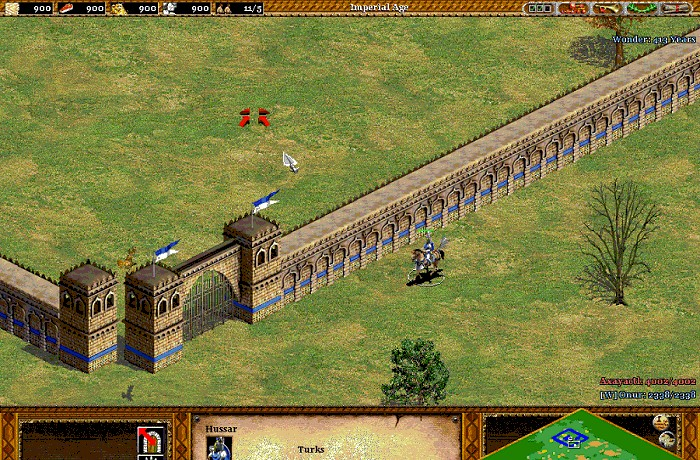
\includegraphics[width=\textwidth]{resimler/ageOfEmpire.jpg}
		\caption{Age of Empires Ekran Al�nt�s�}
		\label{fig:ageOfEmpire}
	\end{subfigure}
	\begin{subfigure}{0.45\textwidth}
		\centering
		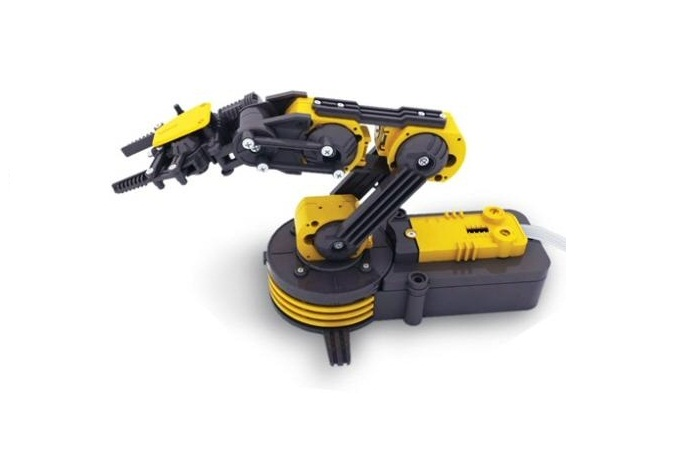
\includegraphics[width=\textwidth]{resimler/robotKolu.jpg}
		\caption{End�striyel Robot Kolu}
		\label{fig:robotKolum}
	\end{subfigure}
\caption{}
\end{figure}

Tam olarak bu nokta, bilgisayar�n ��zmek zorunda oldu�u bir yol planlama problemini ortaya ��kar�r. Bu problemin ��z�m�; ge�ilmez olarak belirlenen engellerden (nehir,orman,binalar gibi) ka��narak, tercihen en k�sa yolu, en k�sa zamanda bulmakt�r. Dikkatli incelendi�inde oyun haritas� ula��labilen veya ula��lamayan kare �eklinde h�crelerden olu�maktad�r. Her bir h�cre yaln�zca oyun i�erisinde bir birimi ta��yabilmekte ve kom�ulu�undaki 8 h�creye ula�abilmektedir. Burada bulunacak yol; kom�u ve ula��labilir h�crelerin birbirlerine ba�lanmas� ile olu�acakt�r.

Bir ba�ka zorlu yol planlama problemi, olas� t�m durumlar�n h�cre yap�s� gibi ayr�k de�ilde s�rekli oldu�u end�striyel robot kollar�n�n (�ekil \ref{fig:robotKolum}) hareketlerinde ortaya ��kar. Bu robot kollar� da, �evrelerindeki herhangi bir engel veya di�er robot kollar� ile �arp��malardan ka��narak �� boyutlu bir ortamda hareket etmektedirler. Bu gibi durumlarda ��z�m, problemi mant�kl� bir �ekilde kolay i�lenebilir hale getirmektir. H�cre y�ntemi kullan�lan bir�ok y�ntemden yaln�zca birisidir. �ki boyut �zerinde bir bilgisayar oyunu ortam� ile �� boyut �zerinde hareket eden end�striyel robot kolu ortam�, farkl� g�r�nseler bile yap�land�rma alanlar� (configuration space) a��s�ndan ayn� genel form�le sahiptirler. Rapor i�eri�inde fabrika y�zeyinde gezinen bir robotun hareketleri modellenirken uygulanan y�ntemlerden bahsedilecektir.\label{giris}
\chapter{Kuramsal Temeller}Yol planlama problemleri, geometrileri ve kordinatlar� de�i�ken hareketli engellerin bulundu�u \emph{Dinamik} ortamlarda ve geometrileri ve kordinatlar� sabit hareketsiz engellerin bulundu�u \emph{Statik} ortamlarda olmak �zere iki farkl� durumda ele al�nabilir. �rne�in bir fabrika i�erisinde gezinen robot kolu, hareketli engel olarak nitelendirebilece�imiz �al��an i��iler ve di�er robot kollar� ile �arp��madan i�lemini ger�ekle�tirmelidir. Ayn� �ekilde bilgisayar oyunu Age of Empires yol planlay�c�s� da dinamik bir �evre �zerinde �al��maktad�r. Di�er bir yandan karma��k bir labirent i�erisinde ��k��� bulmak isteyen bir robot ise statik ortamlarda yol planlama problemini ��zmek zorundad�r. Her iki durum i�in de uygulanabilir y�ntemler mevcuttur. Bu raporda statik ortamlar �zerinde geli�tirilen y�ntemlerden bahsedilecektir.\label{kurumsalTemeller}
	\section{Yap�land�rma Uzay� (Configuration Space)}Yol planlama probleminin olu�abilmesi i�in a�a��da bulunan 4 maddeye ihtiya� vard�r.

\begin{itemize}
	\item Hareket edecek olan nesnenin geometrik �ekli
	\item Nesnenin hareket edece�i �evrenin (workspace\footnote{Workspace nesnenin eri�ebildi�i veya eri�emedi�i t�m yap�land�rmalar� kapsar. Rapor i�eri�inde bu yap� k�saca �evre olarak isimlendirilecektir.}) geometrik tan�mlamas�
	\item Nesne hareketinin serbestlik derecesi tan�mlamas�
	\item Planlanacak olan yolun ba�lang�� ve biti� yap�land�rmalar�
\end{itemize}

Bu maddeler kullan�larak bir robotun yap�land�rma uzay� olu�turulabilir. �rne�in �al��ma alan�ndaki robotun yap�land�rmas�, birka� parametre kullan�larak tan�mlanabilir. 2 boyutlu bir �evre �zerinde �al��an bir robot d���nelim. Bu robotun yap�land�rmas�, bulundu�u y�zeyin x ve y kordinatlar� olarak belirtilebilir. Di�er bir �rnek ile; eklemli robot kollar�n�n yap�land�rmas�n� belirtmek i�in de ard���k ba�lant�lar aras�nda yap�lan a��lar g�sterilebilir. Bir robot yap�land�rmas�n� �zg�n bir �ekilde tan�mlayabilecek, en d���k parametre say�s�na \emph{serbestlik derecesi} (degrees of freedom) denir. ��te bu robot yap�land�rmalar�n�n olu�turdu�u k�meye \emph{yap�land�rma uzay�} ad� verilir ve $\mathcal{Q}$ ile sembollendirilir. K�saca robot kolunun eri�ebilece�i t�m pozisyonlar�n k�mesine yap�land�rma uzay� denir. Robotun serbestlik derecesindeki art��, yap�land�rma uzay�nda da bir art��a neden olur. 

Bir robotun bulundu�u �evrede baz� engeller olabilir. Bu engelleri belirleyen yap�land�rmalar yasakl� (\emph{forbidden}) olarak isimlendirilir. Bir $q$ yap�land�rmas� yasakl� olarak belirlenmi� olsun. Robotun bu yap�land�rmaya gelmesi �evrede bulunan ba�ka bir engel ile �ak��ma durumunu ortaya ��kar�r. Verilen bu $c$ yasakl� yap�land�rma, t�m yasakl� yap�land�rmalar� i�eren $\mathcal{Q}_{forb}$ k�mesinin bir eleman�d�r. Robotun serbest�e gezinebilece�i yap�land�rmalar�n k�mesi de $\mathcal{Q}_{free}$ ile g�sterilir. Yap�land�rma uzay�, serbest ve yasakl� yap�land�rma k�melerinin birle�iminden olu�maktad�r.

Bir yol fonksiyonu, $\pi:[0,L]\rightarrow\mathcal{Q}$ �eklinde s�rekli fonksiyon olarak tan�mlan�r. Burada L yolun uzunlu�unu belirtmektedir. Olu�turulacak yolda �evrede bulunan engellerin hi�biri ile �ak��ma olmamal�d�r. Matematiksel bir �ekilde ifade etmek istersek; ba�lang�� (start) yap�land�rmas� $q_{start}$$\in\mathcal{Q}$ ve hedef (goal) yap�land�rmas� $q_{goal}$$\in\mathcal{Q}$ olan bir �evrede bulunacak yolun �zelli�i: $\pi(0)=$$q_{start}$, $\pi(L)=$$q_{goal}$ olmak �zere $\forall(t\in[0,L]::\pi(t)\in\mathcal{Q}_{free})$ olmal�d�r. K�saca ba�lang�� ve hedef yap�land�rmalar aras�nda ilerlerken ge�ilecek t�m yap�land�rmalar, $\mathcal{Q}_{free}$ k�mesinden se�ilmelidir. Baz� �evrelerde bu �zelliklere sahip birden fazla yol bulunabilir. Bulunan yollar�n birbirinden �st�nl��� mesafelerinin k�sal���yla �l��lebilir.\label{yapilandirmaUzayi}
	\section{Yol Haritalar� (Roadmaps)}B�l�m~\ref{yapilandirmaUzayi} i�erisinde bahsedildi�i gibi yol planlay�c�s�, ba�lang�� ve biti� yap�land�rmalar� aras�nda bir yol planlar. E�er ayn� �evre i�erisinde birden fazla yol bulundu�unu biliyorsak, bu yollar� i�erisinde bar�nd�ran bir veri yap�s� olu�turmak mant�kl� olacakt�r. B�ylece bu veri yap�s� i�erisinden yol daha h�zl� bulunabilir. Olu�turulacak veri yap�s�na \emph{harita} denir. \emph{Haritaland�rma} ise robotun �evresinde olup biteni sens�rleri ile modellemesidir. Robot bulundu�u �evre ile ilgili herhangi bir �nbilgiye sahip olmad��� zamanlarda haritaland�rma �nem kazan�r. Kapal� ortamlarda haritalar�n �� de�i�ik g�sterimleri bulunur: topolojik, geometrik ve h�cresel (bak�n�z �ekil \ref{topoGeometric}).

\begin{figure}[ht]
	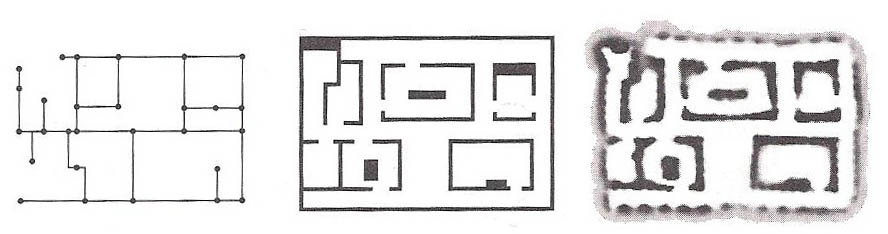
\includegraphics[width=\textwidth]{resimler/topolojikGeotmetrik.jpg}
	\caption{�evrelerin farkl� g�sterimleri: topolojik, geometrik ve h�cresel}\label{topoGeometric}
\end{figure}

Bir \emph{yol haritas�} topolojik harita s�n�f�ndand�r. Yol haritas�nda robotun gidebilece�i se�ilmi� yap�land�rmalar birbiri ile ba�lant�l�d�r ve tamam� $\mathcal{Q}_{free}$ k�mesinden se�ilmi�tir. Rastgele se�ilen bu yap�land�rmalar�n say�s�n�n artmas�, yol haritas�n�n kapsama alan�n� artt�racak ve bulunabilecek yollar aras�nda en k�sa olana yakla��m� sa�layacakt�r. Topolojik bir yol haritas�n�n �zerinde bulunan kenarlar�n ve d���mlerin fiziksel anlamlar� vard�r. �rne�in, bir yol haritas� d���m� eri�ilebilir bir konumu belirler veya iki kom�u d���m aras�nda bulunan �erit bu ikisi aras�ndaki yolu belirler.

Robotlar�n kulland��� yol haritalar� g�nl�k hayatta kulland���m�z otoyol haritalar�na benzemektedir. Gidece�imiz yere varmak i�in t�m sokaklara veya arayollara bakmak yerine hangi anayollar� kullanaca��m�z� belirleriz. Daha sonra ba�lang�� noktam�zdan belirledi�imiz anayola en k�sa yoldan ve ayn� �ekilde hedef noktas�na en yak�n anayoldan ��karak g�zergah�m�z� olu�tururuz. Burada yol haritas� robot i�in anayollar�n bilgisini tutmaktad�r. Bir ba�lang�� yap�land�rmas� $q_{start}$$\in\mathcal{Q}_{free}$ konumundan ba�layan robot ilk �nce kendine en yak�n yol haritas� d���m�ne gitmeli ve daha sonra $q_{goal}$$\in\mathcal{Q}_{free}$ hedep yap�land�rmas�na en yak�n d���mden ��k�p sonuca ula�mal�d�r. Harita �zerinde ise gidilebilecek t�m kom�u yap�land�rmalar �nceden belirlendi�i i�in en k�sa yol algoritmalar� uygulanarak ��k��a en yak�n d���me nerelerden gidilece�i bulunabilir.

\begin{quotation}
\bfseries Yol Haritas� (Roadmap) : \mdseries Serbest yap�land�rma uzay� $\mathcal{Q}_{free}$ i�erisinde bir yol ile ba�lanabilen b�t�n $q_{start}$ ve $q_{goal}$ yap�land�rmalar� i�in a�a��daki �zellikleri sa�layan tek boyutlu e�rilerin olu�turdu�u yap�ya \emph{yol haritas�} (roadmap) denir ve \emph{RM} ile g�sterilir.
\begin{itemize}
	\item Eri�ilebilirlik(Accessibility) : $q_{start}\in Q_{free}$ ko�ulunu sa�layan bir ba�lang�� yap�land�rmas�ndan, $q'_{start}\in$ \emph{RM} ko�ulunu sa�layan baz� yap�land�rmalara giden bir yol bulunmal�d�r.
	\item Ayr�labilirlik(Departability) : $q'_{goal}\in$ \emph{RM} ko�ulunu sa�layan baz� yap�land�rmalardan, $q_{goal}\in Q_{free}$ ko�ulunu sa�layan yap�land�rmaya giden bir yol bulunmal�d�r.
	\item Ba�lanabilirlik : \emph{RM} i�erisinde $q'_{start}$ ve $q'_{goal}$ yap�land�rmalar� aras�nda bir yol bulunmal�d�r.
\end{itemize}
\end{quotation}

Bu �zelliklerden tekinin bile sa�lanmamas�, ba�lang�� ve hedef yap�land�rmalar� aras�nda bir yolun bulunamayaca��n� g�sterir. Bu nedenle yol planlamada do�ru bir yol haritas� olu�turma �nemli yer tutmaktad�r.\label{sec:roadmaps}
	\section{Serbestlik Derecesi (Degrees of Freedom)}Mekanik bir sistemde, yap�land�rmay� olu�turan birbirinden ba��ms�z de�erler �zg�rl�k derecesini (dof \footnote{dof = degrees of freedom}) olu�turur. Bu de�erlerin tamam� bir sistemin durumu hakk�nda bilgiler i�erir. Ayn� zamanda yap�land�rma uzay�n�n boyutunu da belirler. �rne�in fabrikan�n zemininde temizlik yaparak gezinen eklemsiz bir robotu ele alal�m. Bu robotun zemin �zerindeki hareketleri, bulundu�u konumun (x,y) kordinatlar� ile g�sterilebilir.

�zg�rl�k derecesinin boyutu her zaman tek de�i�kenden olu�mayabilir. Ayn� fabrika i�erisinde ara� montaj�nda �al��an 3 eklemli bir robot sisteminin durumu birka� farkl� parametrenin birlikteli�inden olu�ur (�ekil\ref{fig:dof}). Robotun kendi ekseni etraf�nda d�n���, eklemlerin birbirleri ile yapt�klar� a��lar birle�erek sistem yap�land�rmas� hakk�nda bilgi verir.

\begin{figure*}[h]
	\centering
	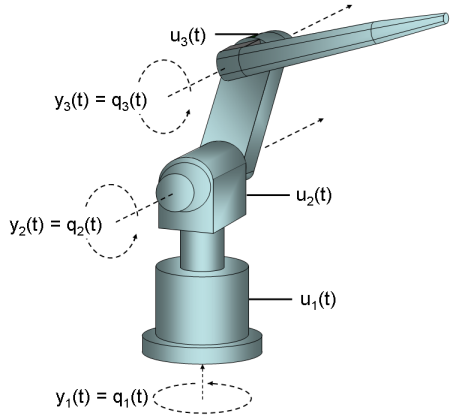
\includegraphics[width=0.30\textwidth]{resimler/dof1.png}
	\hspace{2cm}
	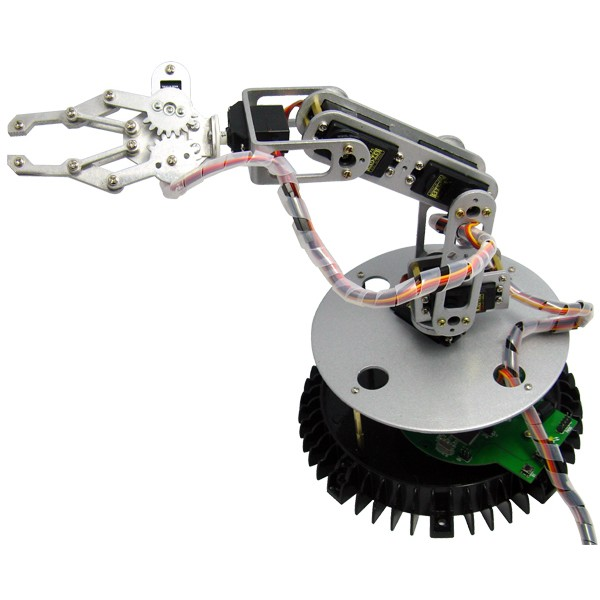
\includegraphics[width=0.30\textwidth]{resimler/dof2.jpg}
	\caption{Degrees of Freedom}
	\label{fig:dof}
\end{figure*}

Robotun kendi ekseni etraf�nda d�n���, t�m kollar�n birbirleri ile yapt�klar� a��lar birle�erek sistemin yap�land�rmas�n� olu�turur. �zg�rl�k derecesinin artmas� $\mathcal{Q}$ yap�land�rma uzay�n�n boyutunu artt�rarak hesaplamalar�n karma��kla�mas�na neden olmaktad�r. B�l�m \ref{chpt:soyp} i�erisinde d�zlem �zerinde gezinen bir robot i�in yol planlama a�amalar�ndan ve kullan�lan algoritmalardan s�z edilecektir.\label{sec:dofs}
	\section{Statik Ortamlarda Yol Planlama}Sadece hareketsiz engellerin bulundu�u ortamlara statik ortamlar denir. �rne�in karma��k labirent i�inde ilerleyen bir robot statik bir ortamda yol planlama problemini ��zmek zorundad�r. Burada bulunulan ortamdaki engellerin boyutlar�, konumlar�, �ekilleri �nceden bilinebilir ya da sens�rler yard�m� ile ilerleme s�ras�nda alg�lanabilir. Bu ayr�mda kullan�lacak metodlarda birbirinden farkl�l�k g�stermektedir. Bu raporda ortamda bulunan engellerin �zelliklerinin �nceden bilindi�i durumlar i�in uygulanan baz� y�ntemler incelenecektir.\label{chpt:soyp}
		\subsection{�rnekleme Tabanl� Y�ntemler}$Q_{free}$ serbest yap�land�rma uzay� i�erisinde yol haritalar� olu�turarak problemleri ��zen bir �ok yol planlay�c�s� bulunmaktad�r. Visibility graph, Cell Decompositions gibi y�ntemlerde bu �ekilde �al��maktad�r. Yap�land�rma uzaylar�n�n boyutlar� artt�k�a bu y�ntemlerin ��z�mleri yetersiz kalmaktad�r. �rnekleme tabanl� y�ntemlerin \emph{(Sample Based Methods)} kullan�m� di�er y�ntemlerin verimli olarak ��zemedi�i, yap�land�rma uzay� boyutunun fazla oldu�u bu tip problemleri ��zmede devreye girmektedir.

�rnekleme tabanl� y�ntemler ilk olarak ortamdan $Q_{free}$ serbest yap�land�rma uzay� i�erisinde olmak �zere yap�land�rmalar toplayarak �n bilgiye sahip olurlar. Daha sonra toplad�klar� bu veriler ile yol planlama problemlerini ��zerler. Yap�land�rma se�imleri rastgele yap�labilece�i gibi \emph{Halton Sequence} veya \emph{Hammersley Sequence} y�ntemleri kullan�larak da yap�labilir. �ekil \ref{fig:randomHalton} 2 boyutlu bir uzay i�erisinde bu y�ntemler kullan�larak elde edilmi� yap�land�rmalar� g�stermektedir.

\begin{figure*}[ht]
	\centering
	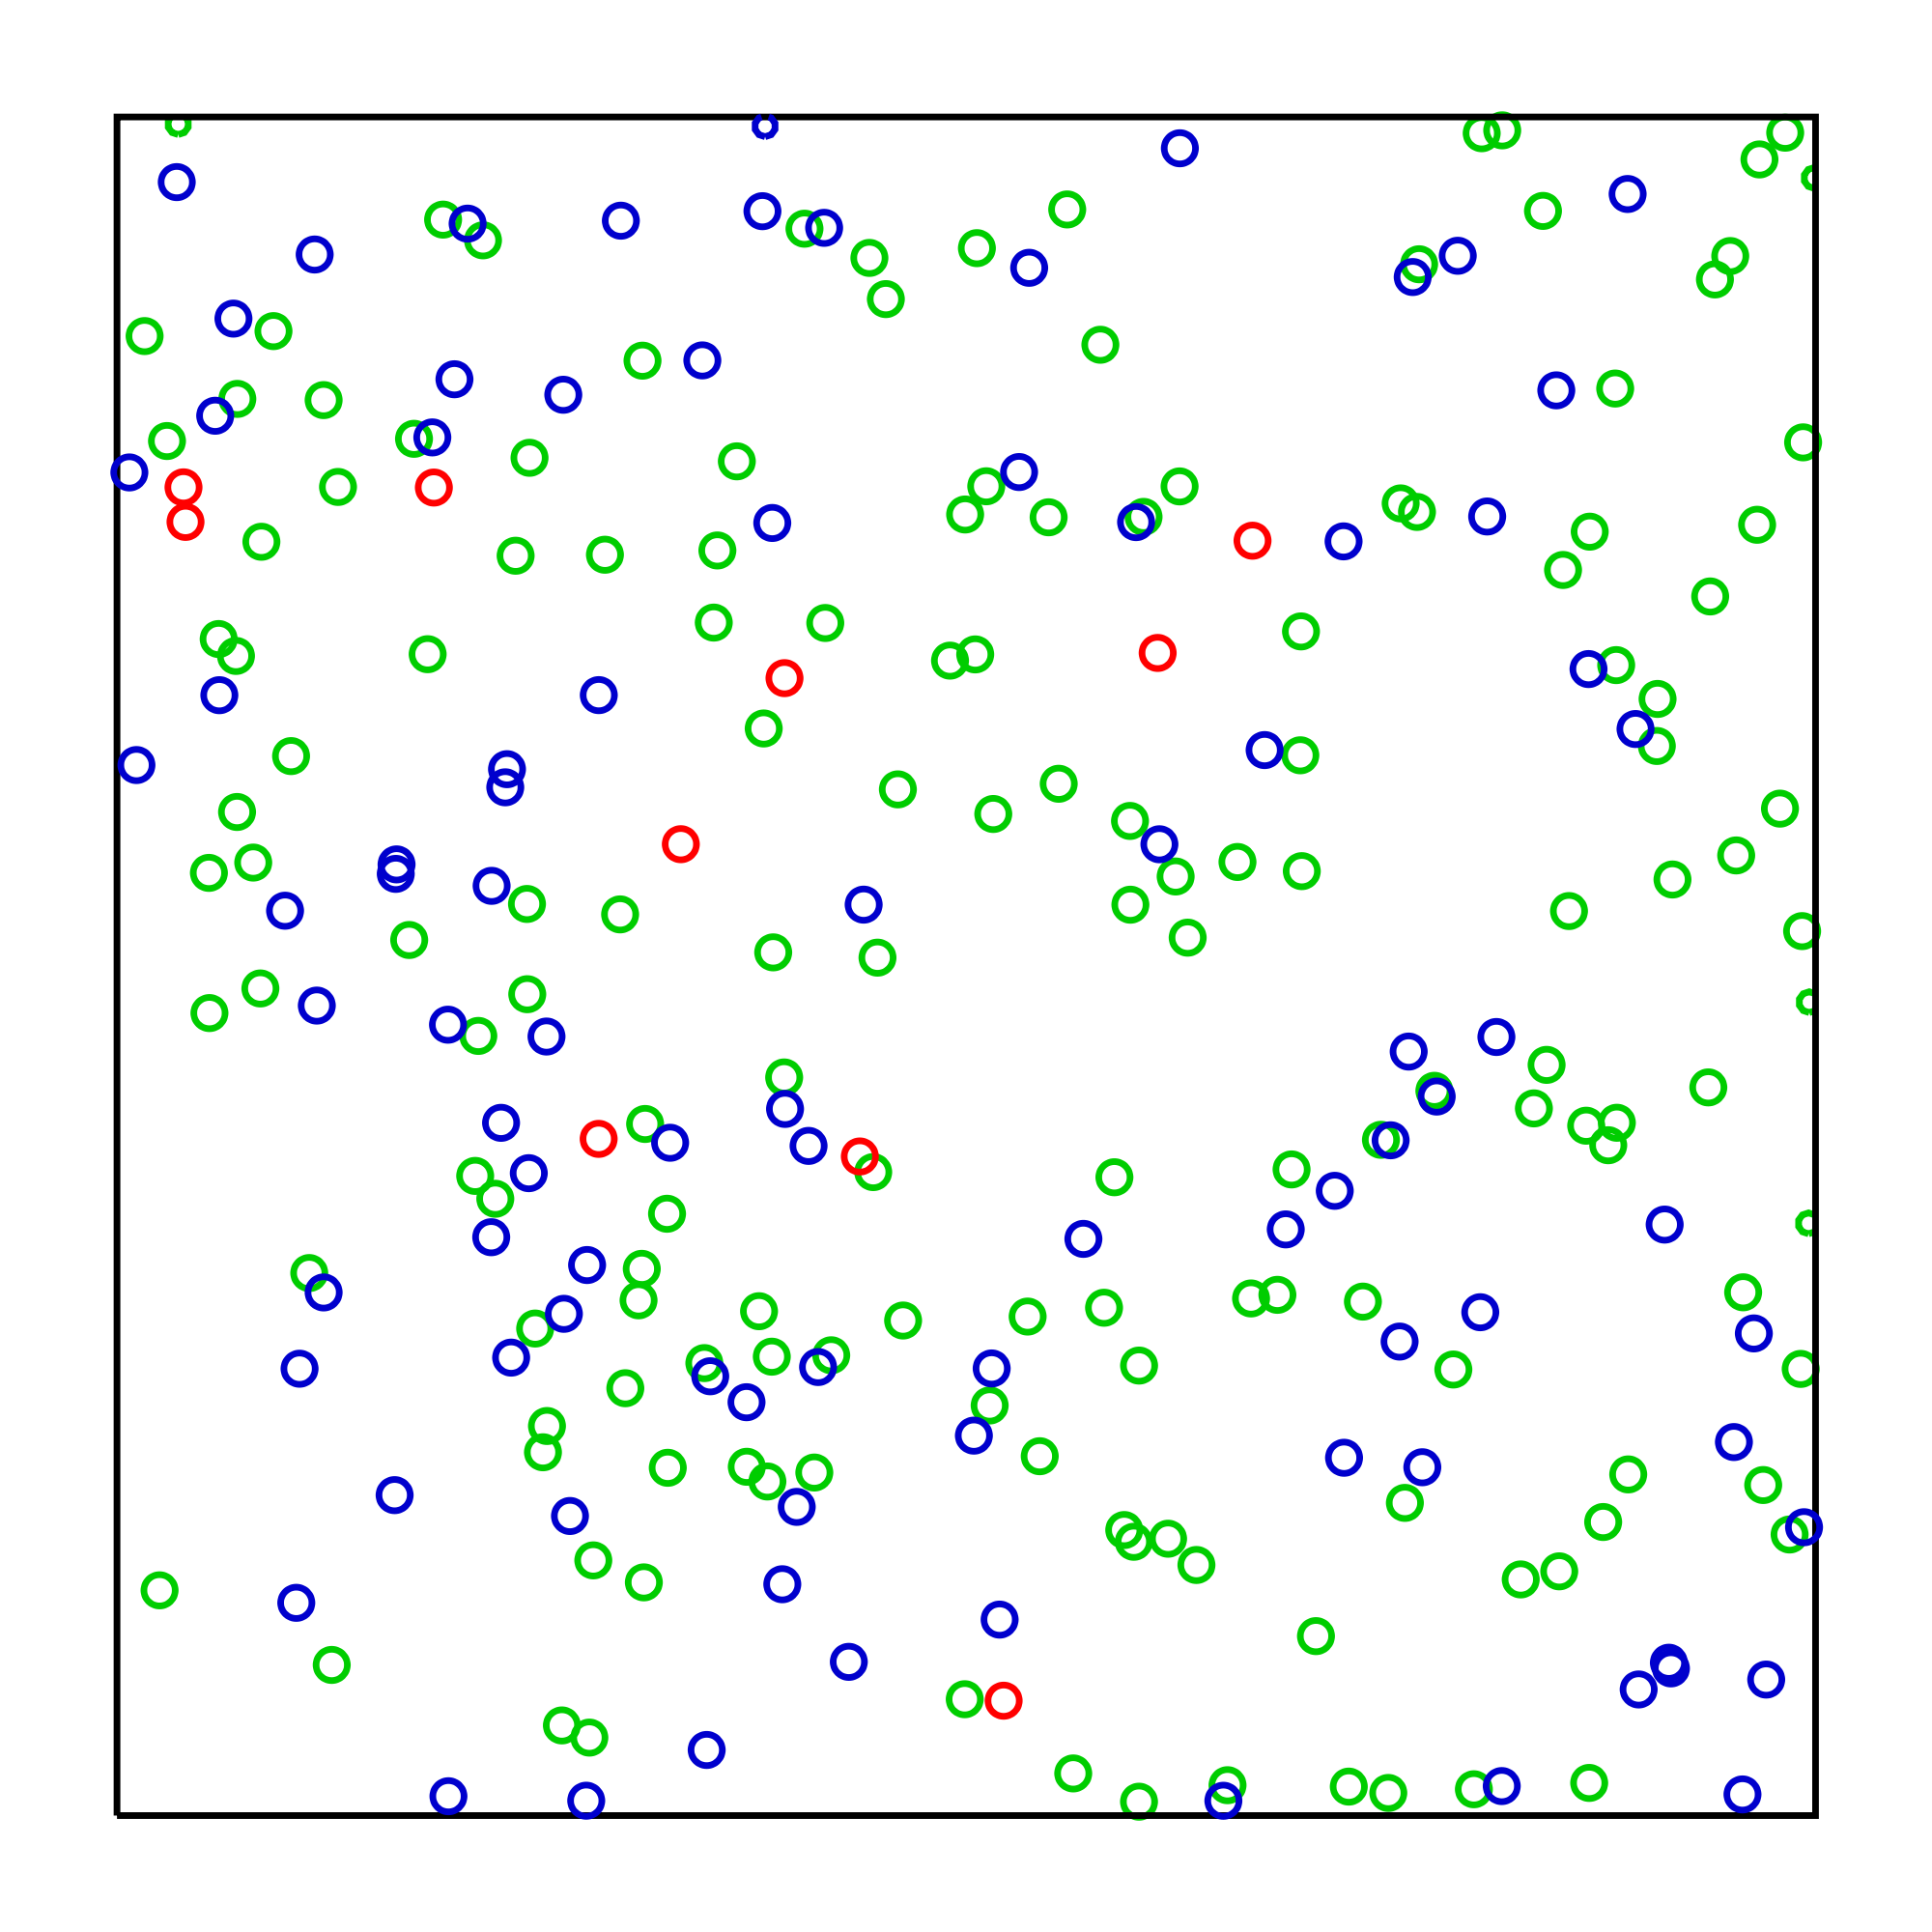
\includegraphics[width=0.30\textwidth]{resimler/random.png}
	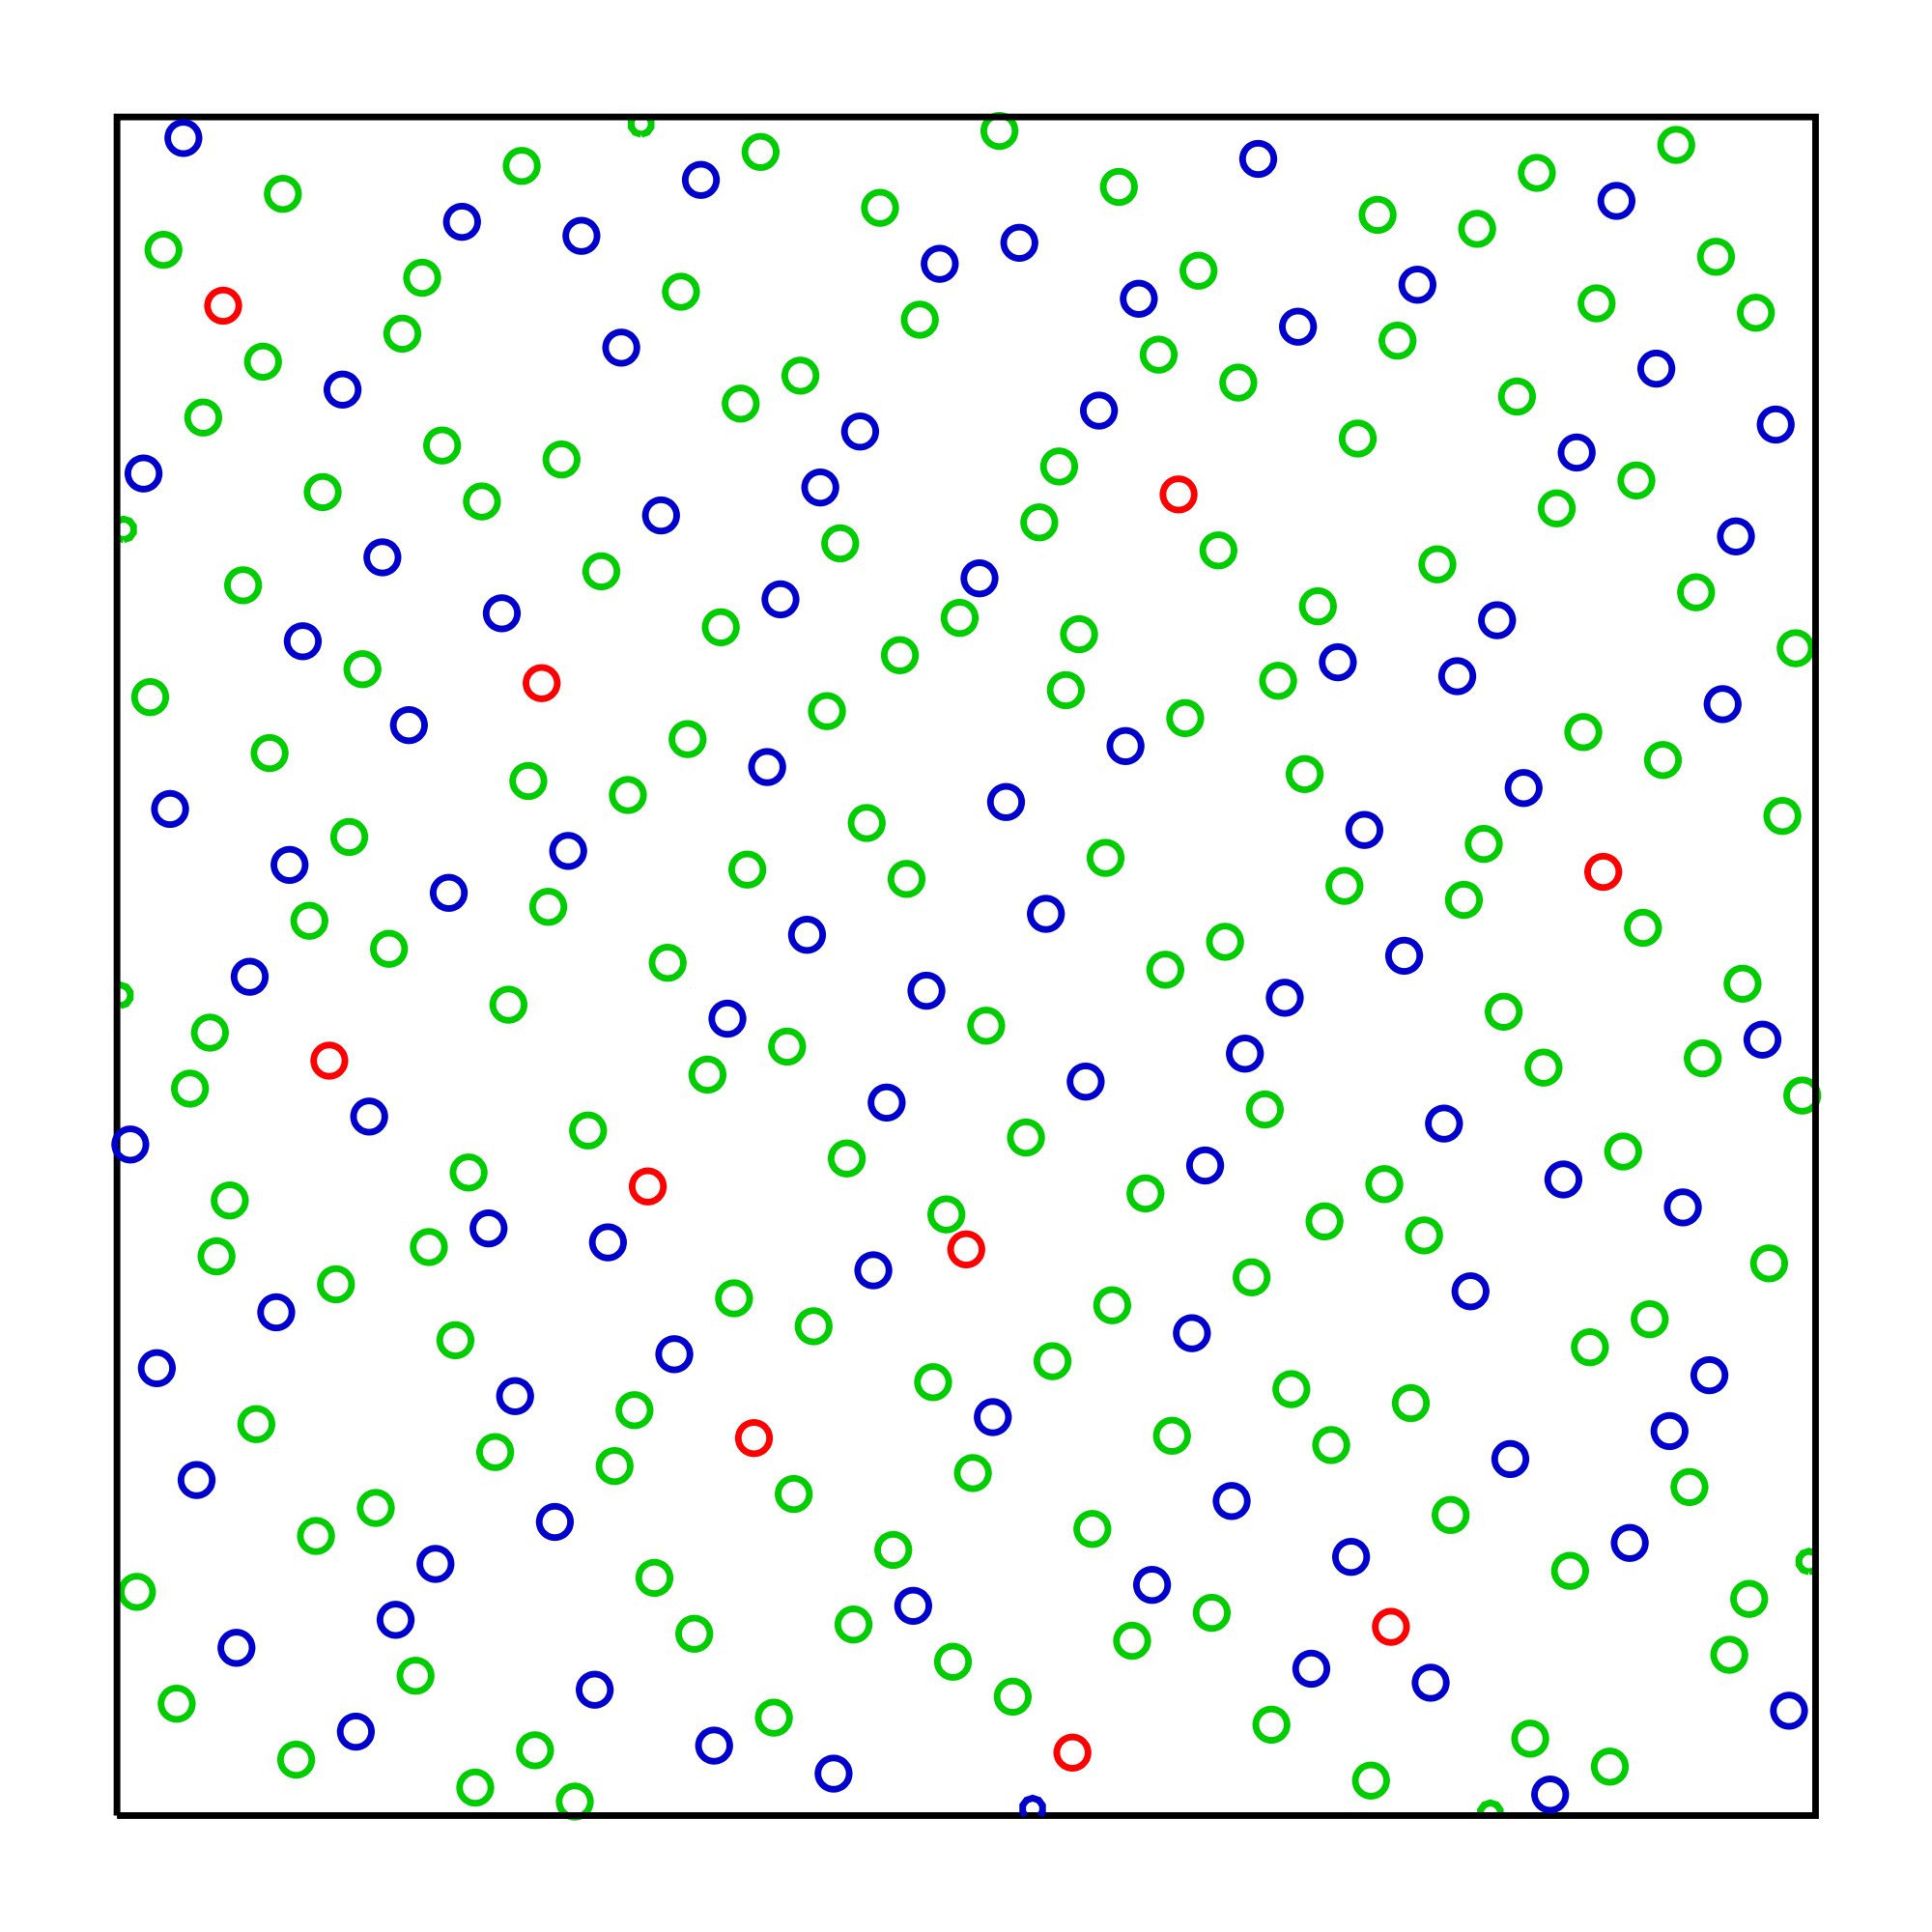
\includegraphics[width=0.30\textwidth]{resimler/halton.png}
	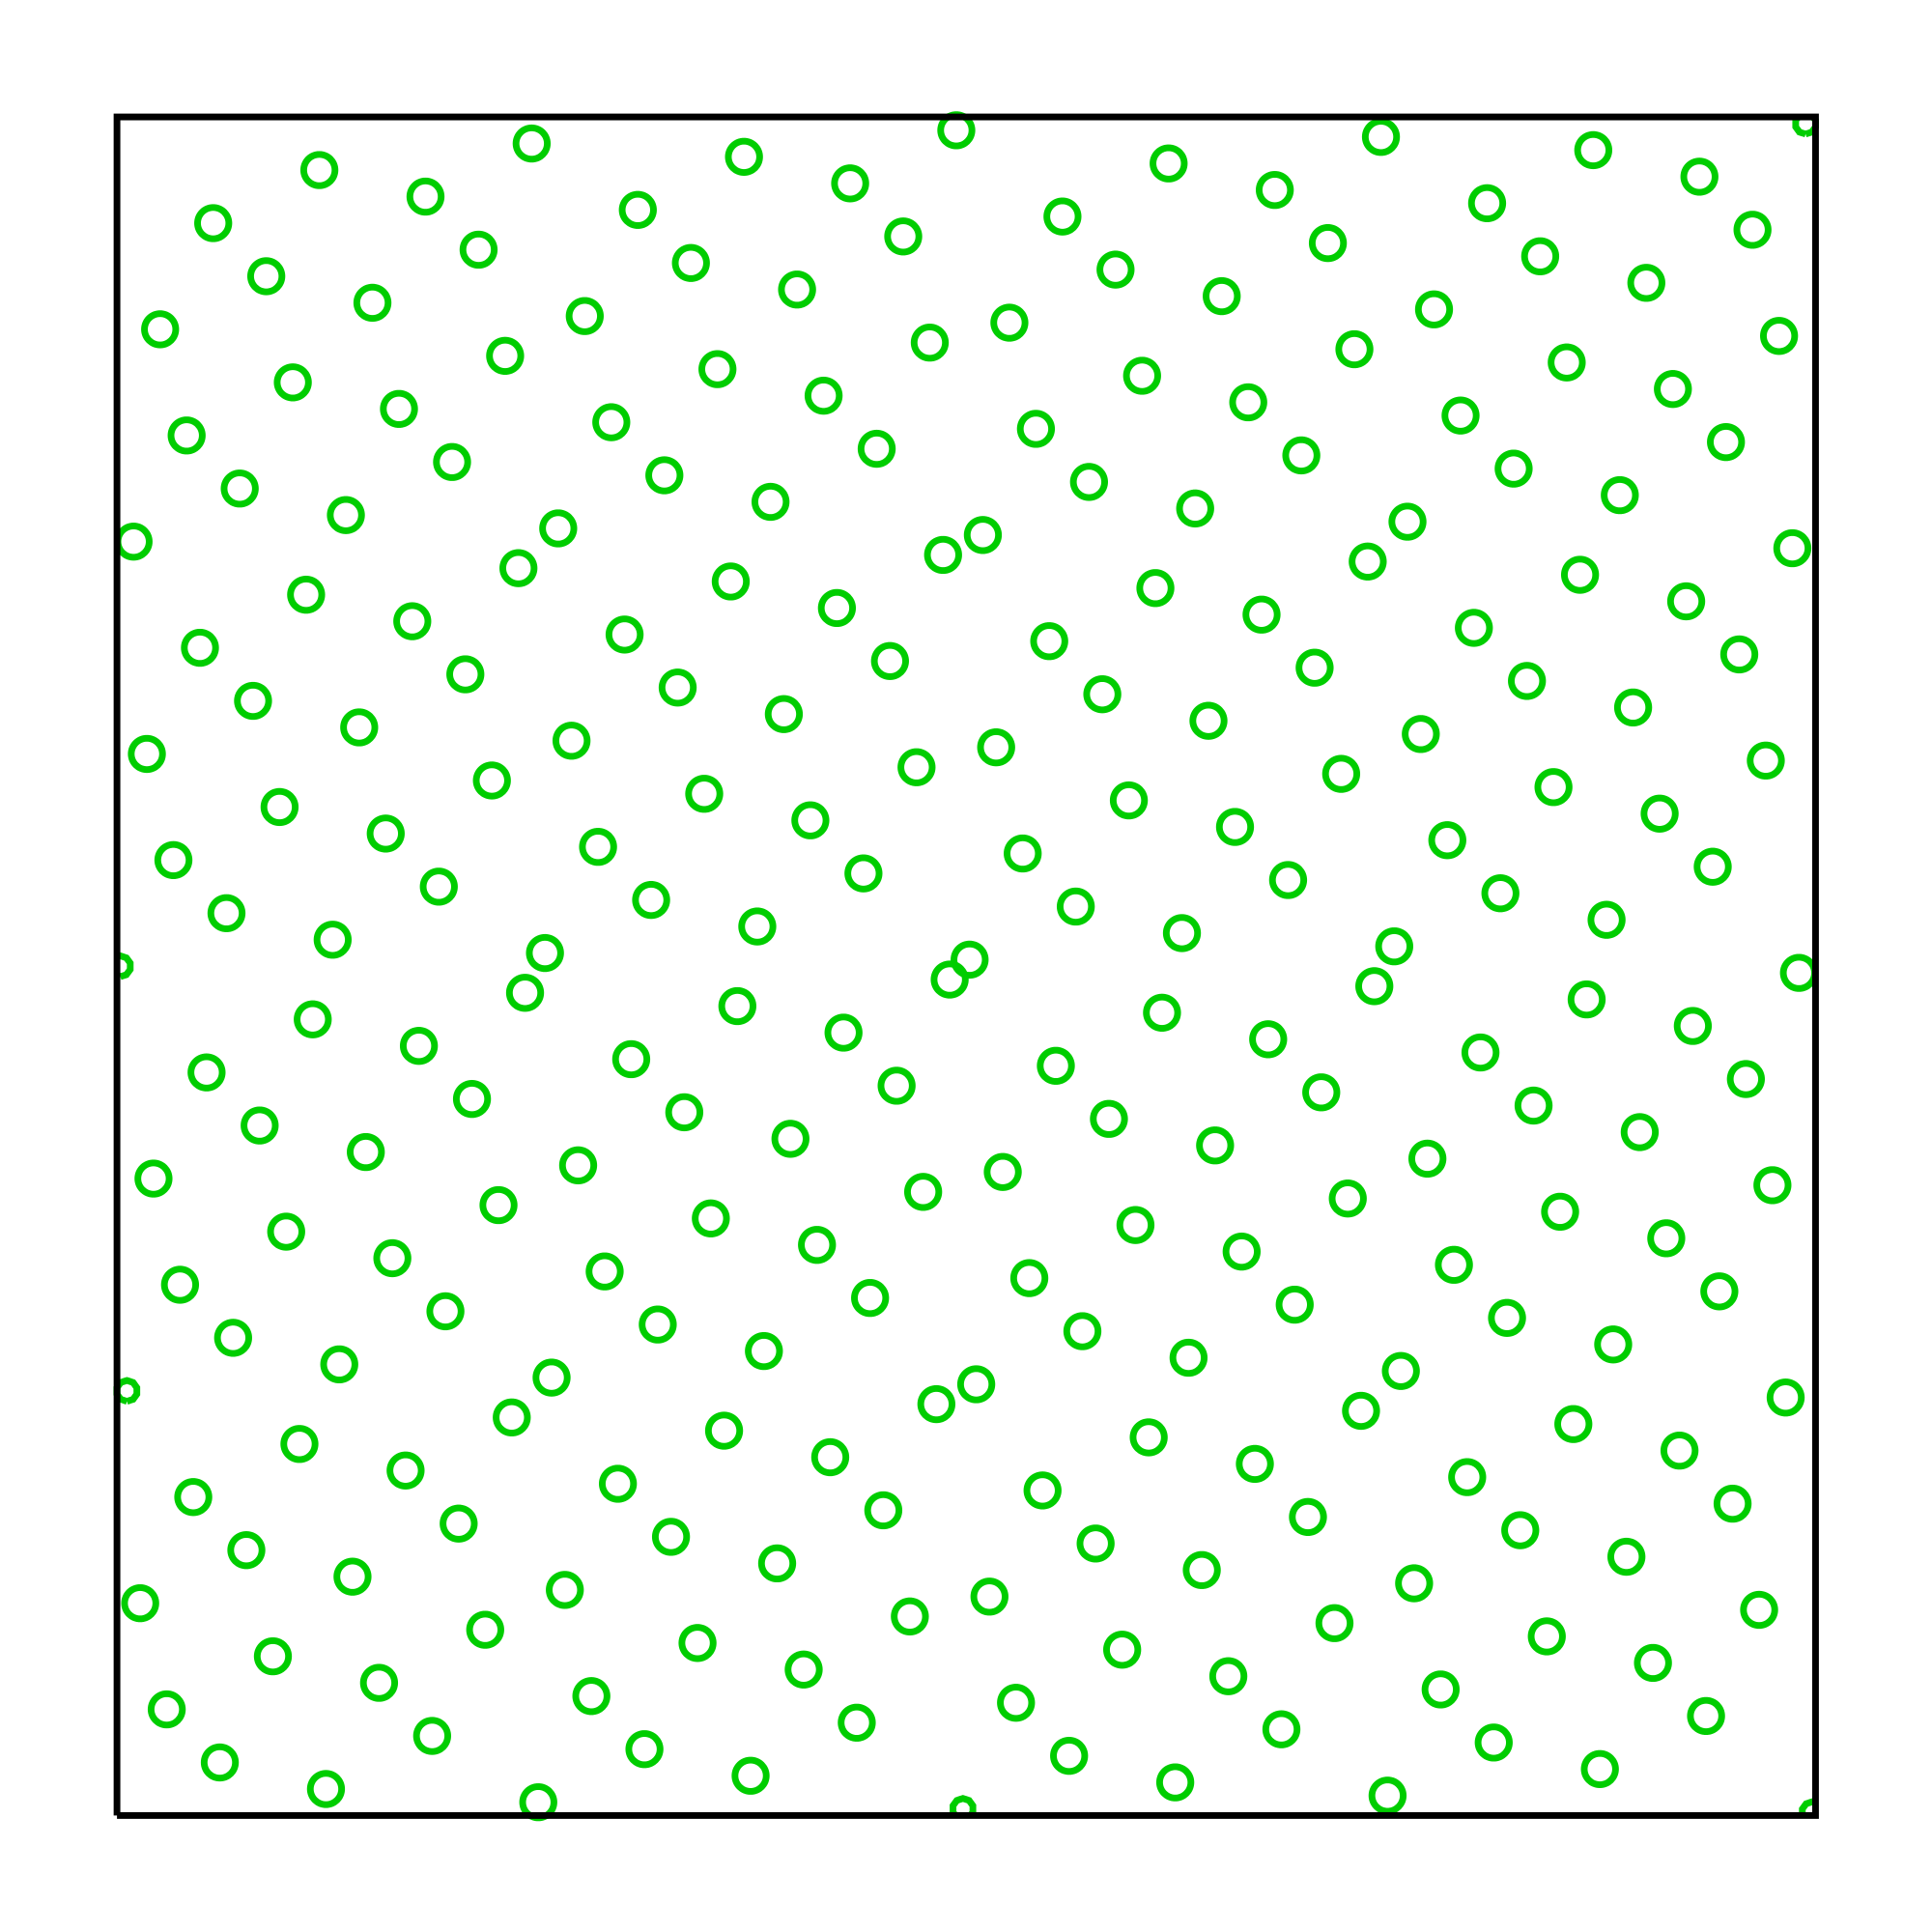
\includegraphics[width=0.30\textwidth]{resimler/hammersley.png}
	\caption{Rastgele, Halton ve Hammersley Y�ntemleri}
	\label{fig:randomHalton}
\end{figure*}\label{subsect:orneklemeTabanli}
		\subsection{Olas�l�ksal Yol Haritalar�}Olas�l�ksal yol haritas� y�ntemi (Probabilistic Roadmap Method\footnote{Rapor i�eri�inde Probabilistic Roadmap Methods yerine PRM k�saltmas� kullan�lacakt�r.}) de �rnekleme tabanl� bir y�ntemdir ve iki safhadan olu�ur. ��renme safhas�nda\footnote{��renme Safhas�(Learning Phase)} robot i�in eri�ilebilir �rnek yap�land�rmalar �retilmektedir. Bu yap�land�rmalar�n tamam� $Q_{free}$ serbest yap�land�rma uzay� i�erisinden se�ilir. Yap�land�rma se�iminin rastgele yap�lmas� bir�ok problem �zerinde etkili olarak �al��maktad�r. Yap�land�rma se�iminin rastgele yap�ld��� bu y�ntemlere temel \emph{(basic)} PRM'ler denir. PRM'in ba�ar�s�, se�ilen bu yap�land�rmalar�n $Q_{free}$ uzay� i�erisinde olup olmad���n�n kontrol�n�n h�z�na da ba�l�d�r. Robotun �zg�rl�k derecesinin artmas� bu kontrolleri karma��k ve zor hale getirecektir. 

PRM, �rnek yap�land�rmalar� elde ettikten sonra bir yol haritas� olu�turacak �ekilde aralar�nda ba�lant� kurmaktad�r. Sorgu safhas�\footnote{Sorgu Safhas� (Query Phase)} olarak adland�r�lan bu safhada, bir yap�land�rmadan di�er bir yap�land�rmaya ba�lant� kurulurken arada ge�ilen t�m yap�land�rmalar�n da $Q_{free}$ k�mesinde bulunma zorunlulu�u vard�r. Bu ko�ullar� sa�layan bir yap� kuruldu�u zaman robotun yapaca�� tek i�lem olu�turulan yol haritas� �zerinde ba�lang�� ve hedef yap�land�rmalar� aras�nda ilerlemek olacakt�r. Olu�turulan bu yol haritas� y�nlendirilmemi� bir �izge $G = (V,E)$ olarak ifade edilir. Burada V, $Q_{free}$ k�mesinden se�ilmi� robot yap�land�rmalar�n� g�stermektedir. E ise e�er varsa iki yap�land�rma ($q_{1}$,$q_{2}$) aras�nda serbest bir yol belirtir.

\begin{algorithm}{}[V,E]
\caption{Yol Haritas� Olu�turma Algoritmas�}
\begin{algorithmic}[1]
\State $V\gets \emptyset$
\State $E\gets \emptyset$
\While{$\mid V \mid < n$}
	\Repeat
		\State $q\gets$Q uzay�ndan rastgele bir yap�land�rma
	\Until{$q \in Q_{free}$}
	\State $V \gets V \cup {q}$
\EndWhile\label{euclidendwhile}
\ForAll{$q \in V$}
	\State $N_{q} \gets$V i�inde uzakl��� g�re se�ilmi� k. kom�u
	\ForAll{$q' \in N_{q}$}
		\If{(q,q') $\notin$ E $ \myAnd \Delta$(q,q') $\neq$ NIL }
			\State $E \gets E \cup$ {(q,q')}
		\EndIf
	\EndFor
\EndFor
\end{algorithmic}
\label{algo1}
\end{algorithm}
Algoritma \ref{algo1} bir yol haritas�n�n olu�turulma s�recindeki t�m a�amalar� g�stermektedir. Ba�lang��ta G = (V,E) �izgesi bo� k�meden olu�maktad�r. Daha sonra $Q$ uzay�ndan bir �rnek yap�land�rma al�n�r. E�er bu yap�land�rma herhangi bir engel ile �ak��ma yapm�yor ise yol haritas�na eklenir. Bu i�lem $Q_{free}$ k�mesinden n say�da yap�land�rma elde edilinceye kadar devam eder. Daha sonra t�m $q \in V$ yap�land�rmalar�ndan $N_{q}$ k elemanl� kom�u k�melerindeki her bir yap�land�rmaya bir yol olup olmad���na bak�l�r. E�er (q,q') aras�nda bir yol bulunabiliyorsa bu yol E k�mesine eklenir. Engellerin �ok s�k bulundu�u ortamlarda $Q$ uzay� i�erisinde n tane �ak��ma olmayan bir yap�land�rma bulma i�lemi zorla�acakt�r. Bu y�zden bu de�erin fazla se�ilmesi bu k�s�mdaki i�lem s�resini art�racakt�r. Az se�ilmesi durumunda ise yap�land�rmalar�n birbirleri ile ba�lant�lar� sa�lanamayacak ve sonu�ta bir yol bulunamayacakt�r.

Bunlar�n yan�nda bir yap�land�rman�n ba�lanaca�� kom�u say�s�n� tan�mlayan k, verimlili�i etkileyen �nemli bir de�i�kendir. Ba�lanacak kom�u say�s�n�n artmas� ba�lanabilirlik testi yap�lacak olan (q,q') �iftlerini art�raca��ndan ek i�lem y�k� getirecektir. Az se�ilmesi ise t�m serbest yap�land�rmalar�n �zerinde bir yol olu�turamayacak kadar d���k elemanl� bir �izge olu�mas�na neden olacakt�r. Bu nedenlerden dolay� n yap�land�rma say�s� ve k kom�u say�s� de�erleri aras�ndaki hassas denge korunmal�d�r. Ba�lanabilirlik testine B�l�m \ref{sect:cakismaAlgilama} i�erisinde de�inilecektir.

\begin{figure}[ht]
	\centering
		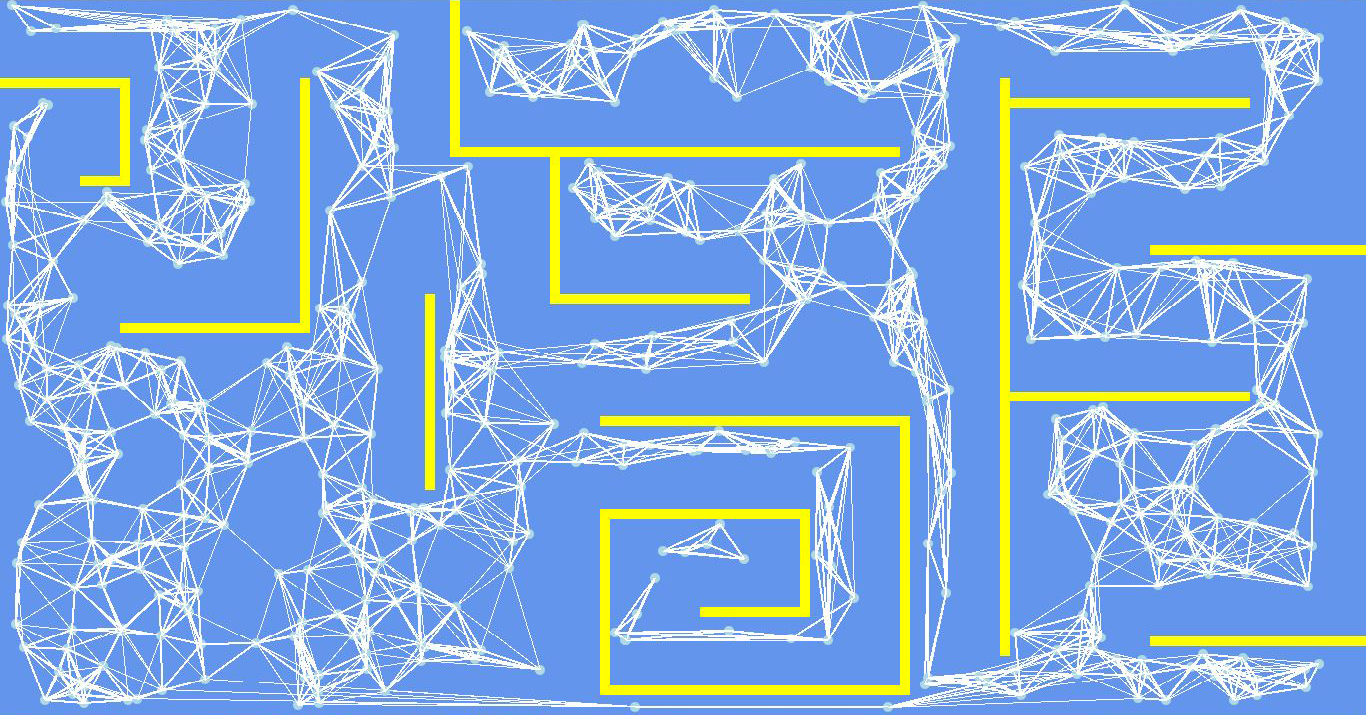
\includegraphics[width=0.80\textwidth]{resimler/roadmapTrue.jpg}
	\caption{2 boyutlu Euclidean uzay�ndaki bir kare i�in yol haritas� uygulamas� }
	\label{fig:roadmapTrue}
\end{figure}

�ekil \ref{fig:roadmapTrue}, XNA Framework\cite{website:xnaFramework} ile yap�lm�� bir yol haritas� uygulamas�n� g�stermektedir. Sar� b�lgeler ortamda bulunan engelleri ifade etmektedir. �rnek yap�land�rmalar�n say�s� n = 500 kabul edilmi� ve ona g�re toplanm��t�r. Her bir yap�land�rma etraf�nda en fazla, ba�lanabilir k = 8 kom�u yap�land�rmaya ba�lanm��t�r. G�r�ld��� gibi neredeyse �o�u dar b�lgelerde ba�lant� sa�lanm��, baz� yap�land�rmalar d��arda kalm��t�r. Ba�lant�lar�n s�rekli oldu�u yap�land�rmalardan kopuk ba�lant�lar�n oldu�u yap�land�rmalara eri�im olmayacakt�r. �rnekleme say�s� veya ba�lanabilir kom�u yap�land�rma say�s� art�r�larak bu istenmeyen durum ortadan kald�rabilir.\label{subsect:olasiliksal}
\chapter{Materyal ve Y�ntem}B�l�m \ref{kurumsalTemeller} i�erisinde anlat�lan bilgiler do�rultusunda, 2 boyutlu d�zlem �zerinde gezinen bir robot sim�lasyonu haz�rlanm��t�r. D�zlem �zerinde statik engeller bulunmaktad�r. Bu sim�lasyon �al��t�r�ld���nda ekranda, pozisyonlar� ve boyutlar� daha �nceden belirtilmi� olan engellerin bulundu�u �evre g�sterilmektedir. Ba�lang�� ve hedef yap�land�rmalar� sim�lasyon �al��ma zaman�nda kullan�c�dan al�nan robot, belirtilen yap�land�rmalar aras�nda engelleri de hesaba katarak en k�sa yolu bulmaya �al��maktad�r. Uygulama Microsoft firmas�n�n sundu�u XNA �at�s� alt�nda C\# programlama dili kullan�larak haz�rlanm��t�r. Bu b�l�mde sim�lasyon ortam�n�n haz�rlanmas� s�ras�nda kullan�lan baz� veri yap�lar�ndan ve y�ntemlerden bahsedilecektir.\label{chap:materyalYontem}
	\section{Pozisyonlar�n Tutulmas�}Sim�lasyon ortam� 2 boyutlu oldu�undan dolay� her cismin x ve y d�zleminde bir pozisyon bilgisi tutulmaktad�r. Ayn� �ekilde en ve boy bilgileri de tutulmal�d�r. Bu nedenle \emph{Position} isiminde s�n�f tan�mlanm��t�r. Position s�n�f� kendi i�inde \emph{leftUpCorner} ve \emph{size} olmak �zere iki de�i�ken bulundurmaktad�r. XNA ortam�n�n sa�lad��� metodlar� da kullanabilmek ad�na bu iki de�i�ken \emph{Vector2} tipinde tutulmaktad�r. B�ylece robotun ekran �zerinde belirlenen bir yerden ba�ka bir yere gitmesi vekt�r i�lemleri ile sa�lanacakt�r.

leftUpCorner; ekranda g�r�nt�lenecek herhangi bir cismin sol �st k��e piksel bilgisini tutmaktad�r. Vector2 veri tipinin kendi i�inde bar�nd�rd��� X ve Y float de�i�kenleri ile cismin ekran �zerinde yerle�imi sa�lanmaktad�r. Benzer �ekilde size de�i�keni de cismin x ve y eksenlerindeki boyutlar�n� belirtecektir. Bu bilgilerin saklanmas�nda Vector2 kullan�m� bar�nd�rd��� metodlar ile olduk�a kolayl�k sa�lam��t�r.

Robotun bulundu�u �evrede engelleri ifade edebilmek i�in \emph{Obstacle} s�n�f� yarat�lm��t�r. Bu s�n�f, bir pozisyon bilgisi ile engelin konumunu ve boyutunu tutmaktad�r. Bunlar�n d���nda ekranda g�sterilecek di�er �zellikleri (renk, isim) de tutulmaktad�r. Engellerin tamam� daha �nceden \emph{Map} s�n�f� alt�nda tan�mlanmaktad�r. Bu s�n�f ortamdaki t�m engelleri \emph{obstacleList} isimli bir Obstacle listesinde tutmaktad�r. Farkl� �evreler yaratabilmek i�in bir de�i�ken yard�m� ile de�i�ik engeller ekranda g�r�nt�lenmektedir.

Sim�lasyonun �al��mas� ba�lad��� anda robot ��renme safhas�na ge�mektedir. Bu safhas�nda gidebilece�i yap�land�rmalar hakk�nda bilgiler toplamaktad�r. Toplad��� bilgilerin saklanmas� i�in \emph{Roadmap} s�n�f tan�mlamas� yap�lm��t�r. Roadmap s�n�f� aktif �evre ve engellerin pozisyonlar�n� tutmaktad�r. Bu s�n�f robot yap�land�rmas�na ba�l� olarak �rnekleme, �rnekleri birbirine ba�lama gibi metodlar �al��t�racakt�r. Bu y�zden \emph{Agent} isimli s�n�f� da tutmaktad�r. Ayr�ca �al��mas� sonucu bir yol haritas� olu�turaca��ndan daha �nceden tan�mlanan Position s�n�f�ndan bir liste tan�mlanm��t�r.\label{sect:pozisyonTutulmasi}
	\section{�ak��ma Alg�lama}Algoritma \ref{algo1} bir yol haritas� olu�turmak i�in gerekli ad�mlar� g�stermektedir. Yol haritas�n� olu�turmaya ba�lamadan �nce $Q_{free}$ serbest yap�land�rma uzay�ndan n say�da �rnekleme al�nmal�d�r. Sim�lasyon bu �rnekleri al�rken rastgele se�imler yapmaktad�r. Her �rnek al�nd���nda, V k�mesine eklemeden �nce se�ilen yap�land�rman�n $Q_{free}$ i�erisinde olup olmad��� kontrol edilmeli e�er bu k�menin elaman� de�ilse yeni bir yap�land�rma se�ilmelidir. E�er bir yap�land�rma hi�bir engel ile �ak��ma yapm�yor ise $Q_{free}$ i�erisindedir. Bu kontrol iki a�amadan olu�maktad�r.

\begin{algorithm}
	\caption{�ki Yap�land�rma Aras�nda �ak��ma Alg�lama}
	\label{algo:intersect}
	\begin{algorithmic}
		\Procedure {Intersect}{$conf1, conf2$}
			\State c1 $\gets$ conf1 yap�land�rmas�n�n merkez noktas�
			\State c2 $\gets$ conf2 yap�land�rmas�n�n merkez noktas�
			\State s1 $\gets$ conf1 yap�land�rmas�n�n boyutlar�
			\State s2 $\gets$ conf2 yap�land�rmas�n�n boyutlar�
			\If {|c1.X - c2.X|<|(s1.X + s2.X)/2| $\And$ |c1.Y - c2.Y|<|(s1.Y + s2.Y)/2|}
				\State \textbf{return} $true$
			\Else
				\State \textbf{return} $false$
			\EndIf
		\EndProcedure
	\end{algorithmic}
\end{algorithm}

�lk a�amada iki yap�land�rma aras�nda bir �ak��ma olup olmad���n� tespit eden bir metod yaz�lm��t�r. Bu metod kendisine parametre olarak gelen iki yap�land�rman�n merkezlerini bulmaktad�r. Merkez pikseli bulunurken sol �st k��enin x ve y d�zlemdeki de�erlerine s�ras�yla en ve boy de�erlerinin yar�s� eklenmektedir. Daha sonra x ekseni �zerinde kesi�me durumu ve y ekseni �zerinde kesi�me durumalar� incelenmektedir (Algoritma \ref{algo:intersect}). E�er her iki eksende birden kesi�me durumu sa�lan�yorsa sonu� do�ru olarak d�ner. Eksenlerden en az birinde kesi�me ko�ulunun sa�lanmamas� durumunda ise kesi�me yoktur denilebilir.

Bu y�ntem ile $Q_{free}$ i�erisinden al�nmas� gereken t�m �rnek yap�land�rmalar toplanmaktad�r. Algoritma \ref{algo:intersect} konumlar� sabit iki yap�land�rman�n �ak��ma yap�p yapmad���n� kontrol etti�inden dolay� rastgele se�ilmi� iki yap�land�rma aras�nda ilerleyen bir Agent nesnesinin, arada kalan b�lgelerde de engellerle kar��la�ma olas�l��� vard�r. Bu y�zden bu ara k�s�mlarda da �ak��ma kontrol� yap�lmal�d�r. Ba�lanabilirlik testi ile bu i�lem ger�ekle�tirilmektedir.

\begin{algorithm}
	\caption{Ba�lanabilirlik Testi}
	\label{algo:confBag}
	\begin{algorithmic}
		\Procedure {isConnectable}{$startConf, goalConf, obstacleList$}
			\State curConf $\gets$ startConf yap�land�rmas� ile ayn�, sanal bir yap�land�rma
			\Repeat
			\State direction $\gets$ curConf - startConf \Comment gidilecek y�n� belirle
			\State curConf $\gets$ curConf + direction \Comment ilerlet
				\ForAll{$obs \in obstacleList$}
					\If{ Intersect(curConf,obs.conf) }
						\State \textbf{return} $false$
					\EndIf
				\EndFor
			\Until{curConf == goalConf}
			\State \textbf{return} $true$
		\EndProcedure
	\end{algorithmic}
\end{algorithm}

Algoritma \ref{algo:confBag}, Agent nesnesinin bir yap�land�rmadan di�er yap�land�rmaya giderken herhangi bir engel ile �ak���p �ak��mad���n� kontrol etmektedir. �lk ba�ta bulunulan yap�land�rman�n bir kopya yap�land�rmas� olu�turulmaktad�r (curConf). Hedef yap�land�rmadan bu yap�land�rma ��kar�l�p normalizasyon i�lemi ger�ekle�tirildi�inde bir y�n de�eri bulunur (direction). Daha sonra curConf yap�land�rmas� goalConf yap�land�rmas�na e�it olana kadar y�n de�eri curConf de�erine eklenerek ilerleme sa�lan�r. �lerlemenin her ad�m�nda curConf yap�land�rmas� �evrede bulunan t�m engellerin yap�land�rmalar� s�rayla Intercest (Algoritma \ref{algo:intersect}) metoduna g�nderilir. Herhangi bir engel ile �ak��ma durumunda Intersect metodundan \emph{true} de�eri d�necektir. B�ylece bu iki yap�land�rman�n ba�lanabilirlik testi ba�ar�z olacakt�r.\label{sect:cakismaAlgilama}
	\section{En K�sa Yolu Bulma}Yol haritas� olu�turulmas� tamamland�ktan sonra robotun gidece�i iki yap�land�rma aras�nda en k�sa yol bulunmal�d�r. Bir �izge �zerinde gezinerek iki d���m aras�nda en k�sa yolu bulan algoritmalardan herhangi biri se�ilebilir. Dijkstra, Bellman-Ford, A* gibi bir�ok algoritma �izgeler �zerinde gezinerek en k�sa yol problemleri i�in ��z�mler �retmektedir. Sim�lasyon uygulamas� haz�rlan�rken $O(|E|\log{|V|})$ �al��ma zaman�na sahip Dijkstra algoritmas� se�ilmi�tir.

\begin{algorithm}
	\caption{Dijkstra}
	\label{algo:dijkstra}
	\begin{algorithmic}
		\Function{Dijkstra}{�izge, ba�lang��}
			\ForAll{d���m $ \in $ �izge}
				\State uzakl�k[d���m] $ \gets \infty$
				\State kaynak[d���m] $ \gets $ NULL
			\EndFor
			
			\State uzakl�k[ba�lang��] $ \gets $ 0
			\State Q $ \gets $ �izge i�indeki t�m d���mler
		
			\While{Q != NULL}
				\State u $ \gets $ Q i�indeki en k�sa uzakl��a sahip d���m
				\State Q $ \gets $ Q - {u}
				\If{uzakl�k[u] == $ \infty $} \Comment Kalan di�er d���mlere eri�ilemez
					\State \textbf{break}
				\EndIf
				\ForAll{ kD���m $ \in $ u.kom�ular }
					\State kisaYol $ \gets $ uzakl�k[u] + (u, kD���m) aras� uzakl�k
					\If { kisaYol < uzakl�k[kD���m] }
						\State uzakl�k[kD���m] $ \gets $ kisaYol
						\State kaynak[kD���m] $ \gets $ u
					\EndIf
				\EndFor
			\EndWhile
		\EndFunction
	\end{algorithmic}
\end{algorithm}

Bu algoritma ile ba�lang�� d���m�nden di�er t�m d���mlere olan uzakl�k belirlenmi�tir. Bu uzakl�klara g�re her d���me en k�sa nerelerden gelindi�i bilgileri de tutulmaktad�r. B�ylece rastgele se�ilen bir d���me giden en k�sa yol bulunabilmektedir.\label{subsect:enKisaYol}
\chapter{Bulgular}B�l�m \ref{chap:materyalYontem} i�erisinden anlat�lan algoritmalara uygun olarak geli�tirilen 2 boyutlu sim�lasyon ortam�nda, PRM yakla��mlar�n�n �al��malar� ile ilgili baz� ��kar�mlar elde edilmi�tir. Bu b�l�mde; sim�lasyon i�erisinde baz� ko�ullar ve durumlar de�i�tirildi�inde elde edilen ��kt�lardaki iyi y�nler ile ortaya ��kan baz� sorunlar ele al�nacakt�r.\label{chpt:bulgular}
	\section{�rnekleme Say�s�n�n Etkisi}Olas�l�ksal yol haritalar� d�zenlenirken al�nan �rnek yap�land�rma say�s� en k�sa yol probleminin ��z�me ula�mas�nda �nemli bir etkendir. �rne�in �evrede hi� engel bulunmayan iki sim�lasyon ortam�n� ele alal�m (�ekil \ref{fig:sampleEtki}). Bu sim�lasyon ortamlar�n�n ilki 500 �rnek yap�land�rma al�narak olu�turulmu� bir yol haritas�n� g�stermektedir. �kincisi ise 10 �rnek al�narak olu�turulmu� bir yol haritas�n� g�stermektedir.

\begin{figure}[h]
	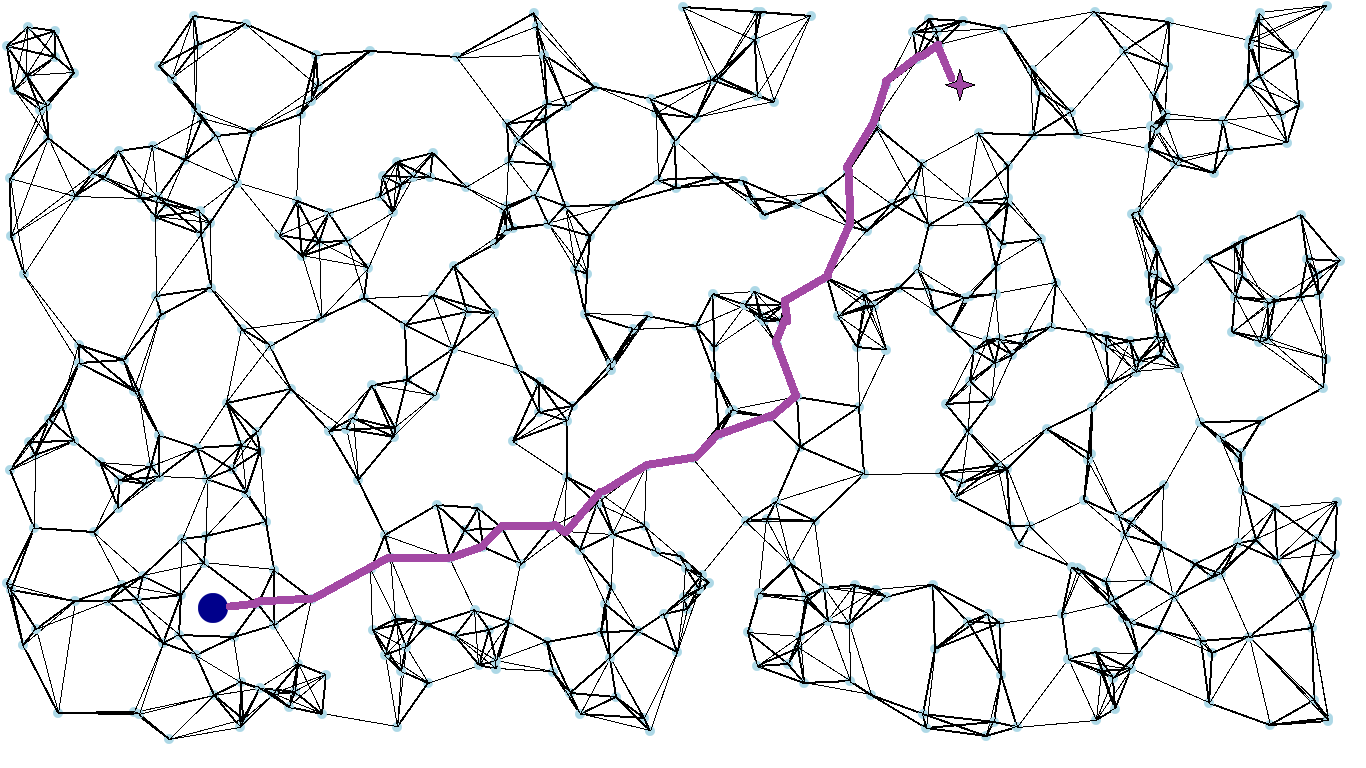
\includegraphics[width=0.47\textwidth]{resimler/sampleEtkisi.png}
	\label{fig:sampleEtkisi1}
	\hspace{5mm}
	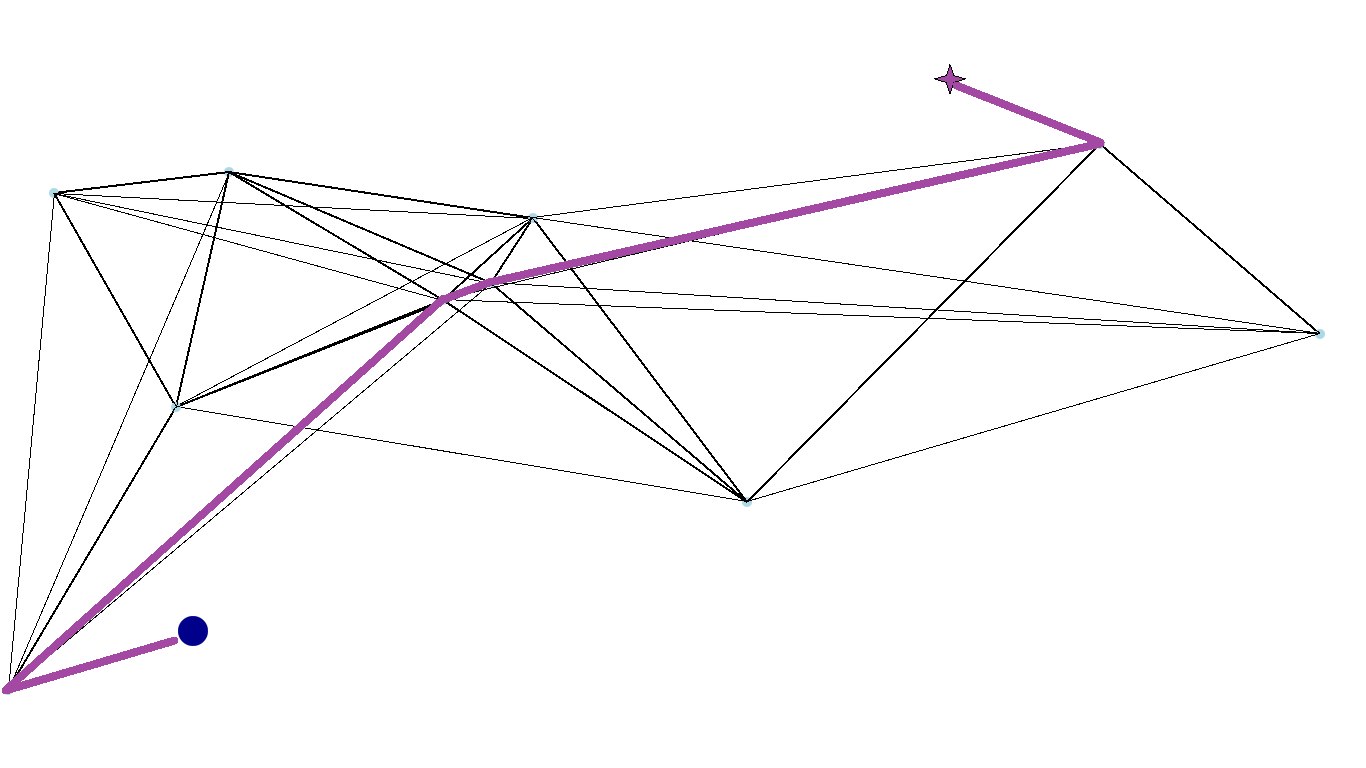
\includegraphics[width=0.47\textwidth]{resimler/sampleEtkisi2.png}
	\label{fig:sampleEtkisi2}
\caption{�rnekleme Say�s�n�n Etkisi}
\label{fig:sampleEtki}
\end{figure}

Al�nan her bir yap�land�rma �evresinde bulunan en fazla 5 kom�u yap�land�rmas�na ba�lanm��t�r. G�r�ld��� �zere yol planlay�c�s� ilk durumda, ikinci duruma g�re daha iyi bir yol bulabilmi�tir. 10 �rnek al�nan sim�lasyon ortam�nda hareket eden cisim ba�lang�� pozisyonundan ��karak yol haritas�na en yak�n d���me gitmeye �al��m��t�r. Bu da yolun uzamas�na neden olmu�tur. Bu �rnek, al�nan �rnek yap�land�rma say�s� ile en iyi yola yakla��m�n do�ru orant�l� oldu�unu g�stermektedir.

\begin{figure}[h]
	\centering
	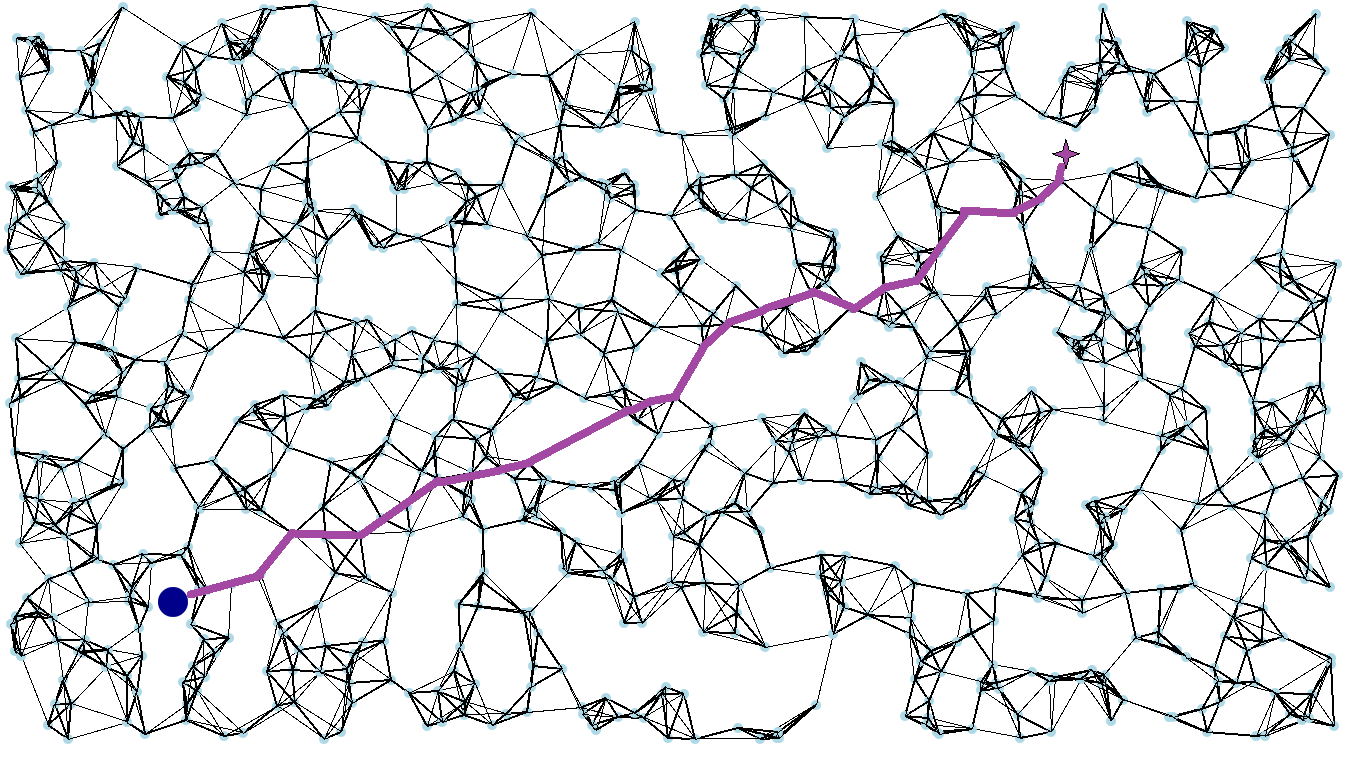
\includegraphics[width=0.70\textwidth]{resimler/sampleEtkisi3.png}
	\caption{1000 �rnek yap�land�rmal� PRM}
	\label{fig:sampleEtkisi3}
\end{figure}

�ekil \ref{fig:sampleEtkisi3} di�er de�i�kenler sabit tutulup 1000 �rnek al�narak olu�turulan bir yol haritas�n� g�stermektedir. Burada hareketli cisim ba�lang�� ve hedef yap�land�rmas� aras�da neredeyse d�z bir hat �zerinde ilerleyerek en k�sa yoldan gitmi�tir. Fakat bu sim�lasyon �rne�inde yol haritas�n�n olu�turulmas� daha uzun bir zaman alm��t�r. �rnekleme say�s�n�n art�r�lmas� �al��ma zaman�n�n uzamas�na da neden olmu�tur.



\label{sect:orneklemeEtkisi}
	\section{Kom�u Say�s�n�n Etkisi}Bir yol haritas� olu�turulurken herhangi bir d���mden ula��labilecek kom�u d���mlerin say�s�n�n artmas� hem ba�lanabilirlik testinde, hemde Dijkstra algoritmas�nda ek i�lem yap�lmas�na neden olacakt�r. Bu de�i�kenin etkilerini g�rebilmek i�in �rnekleme say�s�n�n sabit tutuldu�u iki sim�lasyon ortam�n� ele alal�m (�ekil \ref{fig:komsuEtki}).

\vspace{-1mm}
\begin{figure}[h]
	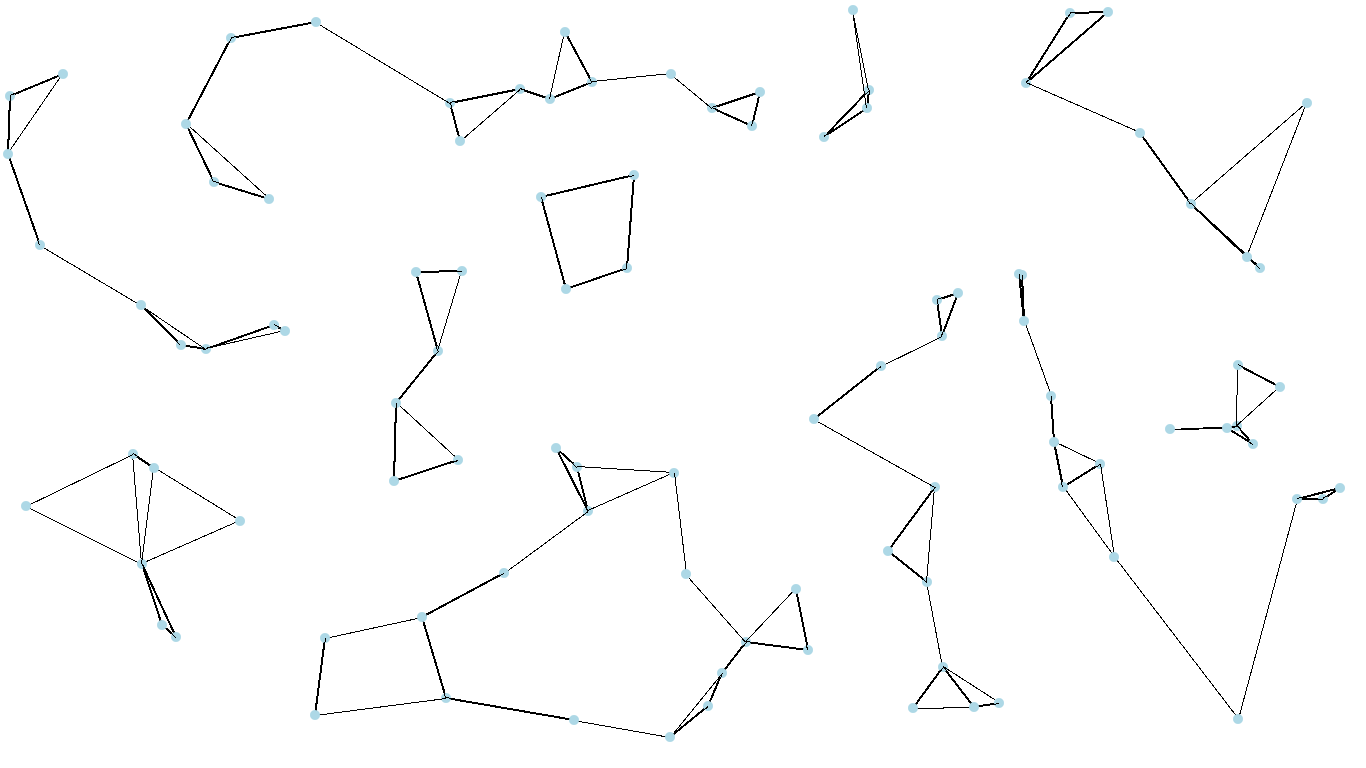
\includegraphics[width=0.47\textwidth]{resimler/komsuEtkisi.png}
	\label{fig:komsuEtkisi1}
	\hspace{5mm}
	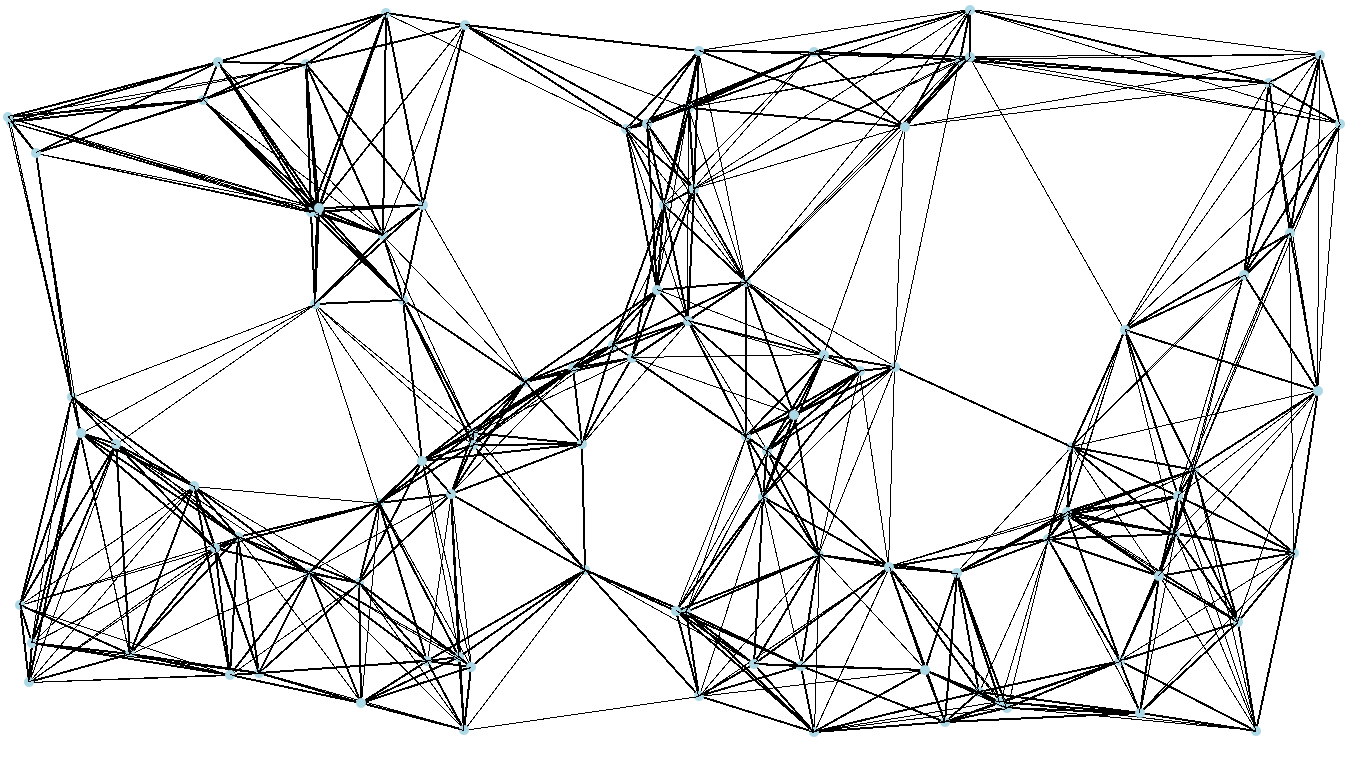
\includegraphics[width=0.47\textwidth]{resimler/komsuEtkisi2.png}
	\label{fig:komsuEtkisi2}
\caption{Kom�u Yap�land�rma Say�s�n�n Etkisi}
\label{fig:komsuEtki}
\end{figure}

�lk �rnekte ba�lanabilir kom�u yap�land�rma say�s� 2 olarak ayarlanm��t�r. B�ylece her yap�land�rma kendine yak�n en fazla 2 yap�land�rmaya ba�lanm��t�r. Bu y�zden �izge �ok say�da alt �izgelere ayr�lm�� ve b�t�nl�k sa�lanamam��t�r. Bu durumda herhangi iki yap�land�rma aras�nda eri�im sorunlar� olu�acakt�r. �kinci �rnekte �rnekleme say�s� sabit tutularak ba�lanabilir kom�u say�s� 10'a ��kar�lm��t�r. Bu durum her bir d���m i�in uygulanacak ba�lanabilirlik testi say�s�n� 5 kat daha artt�rm��t�r. Bu y�zden yol haritas�n�n olu�turulmas� daha uzun s�rm��t�r.\label{sect:komsuSayisi}
	\section{Engellerin Etkisi}Ortamda bulunan engellerin artmas� $Q_{free}$ yap�land�rma k�mesinin eleman say�s�n� azaltmaktad�r. Bu y�zden robotun gidebilece�i yap�land�rmalar�n say�s� azalmakta ve hareketleri k�s�tlanmaktad�r. �rnekleme ve kom�u yap�land�rma say�s�n�n ayn�, biri engel yo�unlu�unun az ve di�erinin daha yo�un engellerden olu�tu�u iki sim�lasyon ortam�n� ele alal�m.

\begin{figure}[h]
	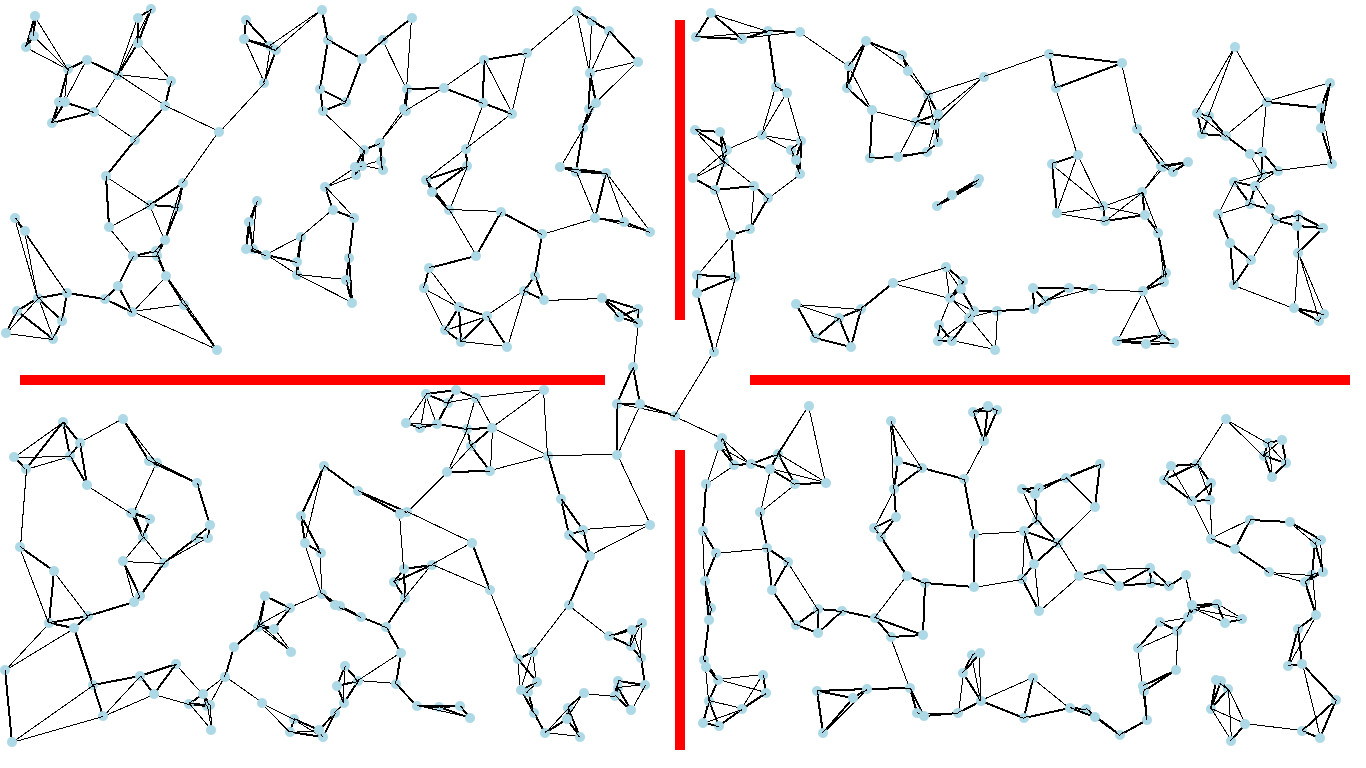
\includegraphics[width=0.47\textwidth]{resimler/500ornek3komsuMap2.png}
	\label{fig:mapEtkisi1}
	\hspace{5mm}
	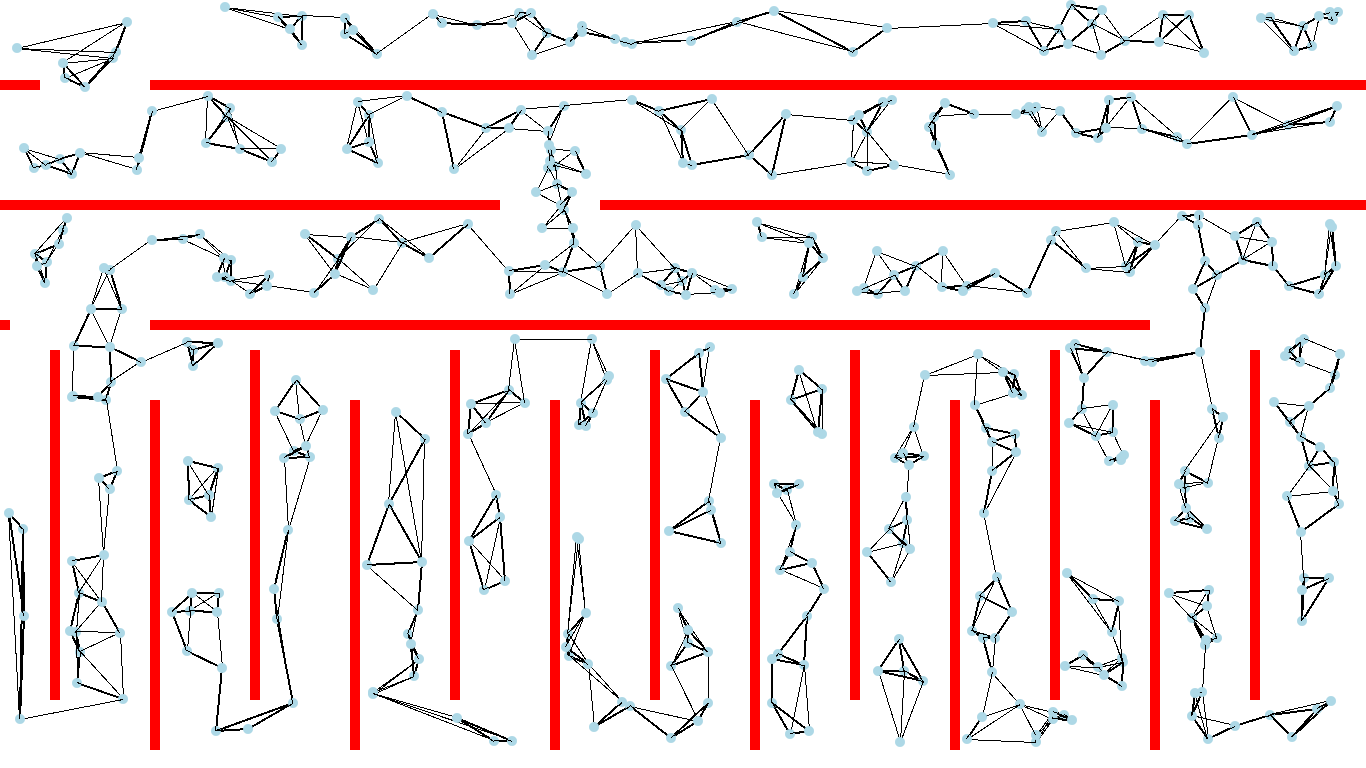
\includegraphics[width=0.47\textwidth]{resimler/500ornek3komsuMap1.png}
	\label{fig:mapEtkisi2}
\caption{Engellerin Etkisi}
\label{fig:mapEtki}
\end{figure}

�ekil \ref{fig:mapEtki} i�inde bulunan iki sim�lasyon �rne�i 500 �rnek yap�land�rma al�narak ve her yap�land�rma 3 kom�usuna ba�lanarak olu�turulmu�tur. G�r�ld��� �zere ilk �rnekte engellerin bulunma s�kl��� az oldu�undan, olu�turulan yol haritas� �zerinde kopukluklar nadir g�r�lm��t�r. $Q_{free}$ yap�land�rma k�mesinin neredeyse tamam�na eri�im sa�lanmaktad�r. �kinci �rnekte ise engeller s�k g�r�ld���nden al�nan �rneklerin birbirine ba�lanmas�nda s�k�nt�lar ya�anm��t�r. Engeller aras�nda bulunan dar bo�az ge�i�lerde kopukluklar ya�anm�� ve b�t�n bir yol haritas� olu�turulamam��t�r.

Engellerin s�k oldu�u bu t�r ortamlarda �rnekleme say�s�n� art�rmak tam bir yol haritas� olu�turmak i�in iyi bir ��z�md�r fakat ba�lanabilir kom�u yap�land�rma say�s� da do�ru �ekilde ayarlanmal�d�r. �ekil \ref{fig:3000ornek5komsu} engellerin bulundu�u bir ortam i�in 3000 �rnek yap�land�rma al�narak olu�turulmu� bir yol haritas�n� g�stermektedir. Her yap�land�rma �evresinde bulunan 3 kom�u yap�land�rmas�na ba�lanm��t�r.

\begin{figure}[ht]
	\centering
		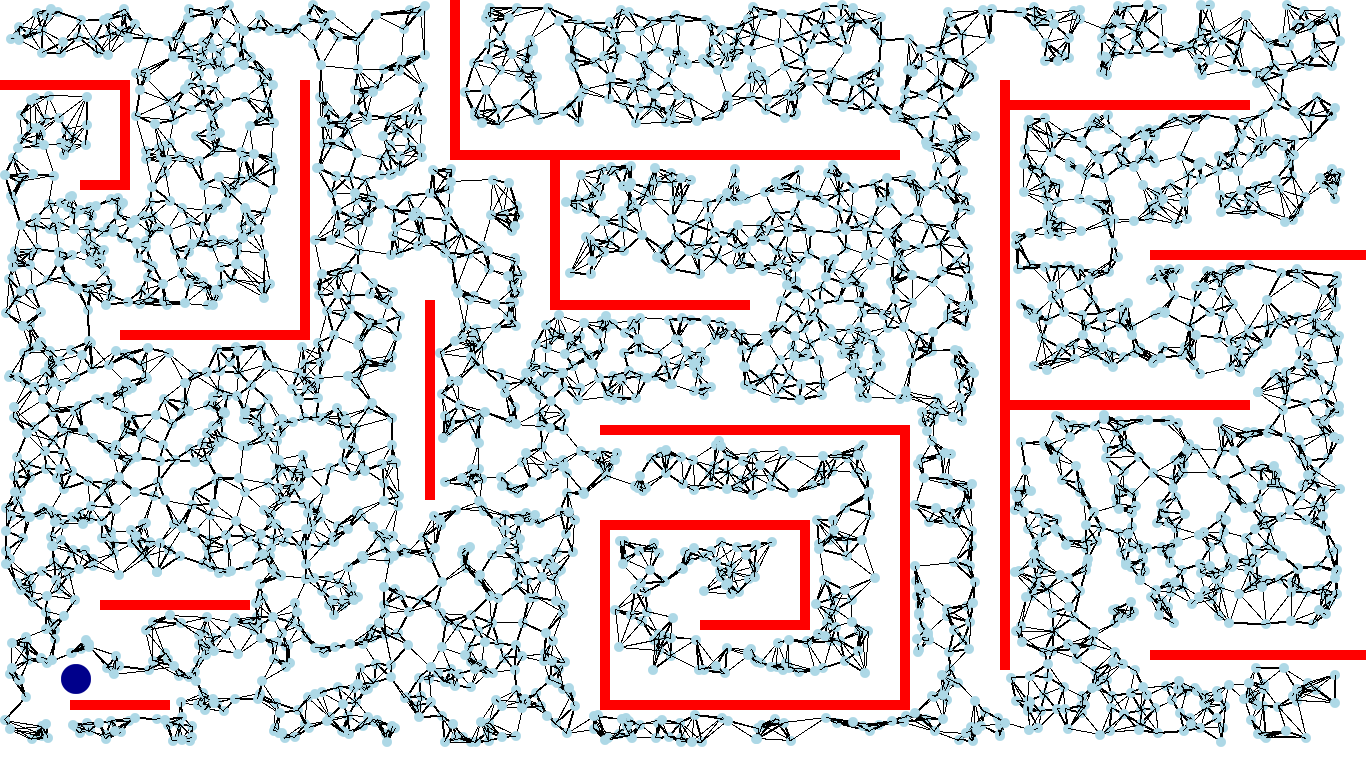
\includegraphics[width=0.70\textwidth]{resimler/3000ornek5komsu.png}
	\caption{3000 �rnek yap�land�rma al�narak olu�turulmu� yol haritas� �rne�i}
	\label{fig:3000ornek5komsu}
\end{figure}

Yol haritas�n�n olu�turulmas� s�ras�nda al�nan �rneklerden baz�lar� $Q_{forbidden}$ yasakl� yap�land�rmalar k�mesinin eleman�d�r. Bu elemanlar�n se�iminde �ak��ma alg�lama testi negatif sonu� d�nd�rmekte ve yerine yeni bir yap�land�rma se�imi daha yap�lmaktad�r. Her yap�land�rma se�im i�lemi programa ek i�lem y�k� getirmekte ve �al��ma zaman�n� k�t� y�nde etkilemektedir. Ayr�ca 3000 �rnek yap�land�rman�n t�m kom�ular�na ba�lanabilirlik testi uygulanmaktad�r. Bu test de �rnekleme say�s�na ba�l� olarak �al��ma zaman�n� etkilemektedir.\label{sect:engelEtkisi}
\chapter{Tart��ma ve Sonu�}


%%%%%%%%%%%%%%%%%%%%%%%%%%%%%%%%%%%%%%%%%%%%%%%%%%%%%%%%%%%%%
%% BIBLIOGRAPHY AND OTHER LISTS
%%%%%%%%%%%%%%%%%%%%%%%%%%%%%%%%%%%%%%%%%%%%%%%%%%%%%%%%%%%%%
%% A small distance to the other stuff in the table of contents (toc)
\addtocontents{toc}{\protect\vspace*{\baselineskip}}

%% The Bibliography
%% ==> You need a file 'literature.bib' for this.
%% ==> You need to run BibTeX for this (Project | Properties... | Uses BibTeX)
%\addcontentsline{toc}{chapter}{Bibliography} %'Bibliography' into toc
%\nocite{*} %Even non-cited BibTeX-Entries will be shown.
%\bibliographystyle{alpha} %Style of Bibliography: plain / apalike / amsalpha / ...
%\bibliography{literature} %You need a file 'literature.bib' for this.

%% The List of Figures
%\clearpage
%\addcontentsline{toc}{chapter}{List of Figures}
%\listoffigures

%% The List of Tables
%\clearpage
%\addcontentsline{toc}{chapter}{List of Tables}
%\listoftables


%%%%%%%%%%%%%%%%%%%%%%%%%%%%%%%%%%%%%%%%%%%%%%%%%%%%%%%%%%%%%
%% APPENDICES
%%%%%%%%%%%%%%%%%%%%%%%%%%%%%%%%%%%%%%%%%%%%%%%%%%%%%%%%%%%%%
%\appendix
%% ==> Write your text here or include other files.

%\input{FileName} %You need a file 'FileName.tex' for this.

\addtocontents{toc}{\protect\vspace*{\baselineskip}}
\clearpage
\addcontentsline{toc}{chapter}{Kaynak�a}
\nocite{*} 
\bibliographystyle{plain}
\bibliography{refs}	
\end{document}

